\documentclass[10pt,a4paper]{report}
\usepackage[utf8]{inputenc}
\usepackage[T1]{fontenc}
\usepackage[english]{babel}
\usepackage{geometry}
\usepackage{graphicx}
\usepackage{hyperref}
\usepackage{listings}
\usepackage{xcolor}
\usepackage{longtable}
\usepackage{booktabs}
\usepackage{fancyhdr}
\usepackage{titlesec}
\usepackage{enumitem}
\usepackage{url}
\usepackage{tabularx}
\usepackage{multirow}
\usepackage{tikz}
\usetikzlibrary{shapes.geometric, arrows.meta, positioning, fit, backgrounds, calc}

% Page geometry
\geometry{
    left=2.5cm,
    right=2.5cm,
    top=3cm,
    bottom=3cm,
    headheight=15pt
}

% Hyperref setup
\hypersetup{
    colorlinks=true,
    linkcolor=blue,
    filecolor=magenta,
    urlcolor=cyan,
    citecolor=green,
    pdftitle={Final Project Report - The Hive Platform},
    pdfauthor={Sena Oz, Aysenur Unal, Kenan Altunbas, Yusuf Savas}
}

% Code listing setup
\lstset{
    basicstyle=\ttfamily\small,
    breaklines=true,
    frame=single,
    numbers=left,
    numberstyle=\tiny\color{gray},
    backgroundcolor=\color{gray!10},
    keywordstyle=\color{blue},
    commentstyle=\color{green!60!black},
    stringstyle=\color{red},
    showspaces=false,
    showstringspaces=false
}

% Header and footer
\pagestyle{fancy}
\fancyhf{}
\fancyhead[L]{\leftmark}
\fancyhead[R]{\thepage}
\fancyfoot[C]{SWE 574, Spring 2026 --- Final Project Report}

% Title formatting
\titleformat{\chapter}[display]
{\normalfont\Large\bfseries}{\chaptertitlename\ \thechapter}{20pt}{\Large}
\titlespacing*{\chapter}{0pt}{50pt}{40pt}

\begin{document}

% Title page
\begin{titlepage}
    \centering
    \vspace*{2cm}
    {\Huge\textbf{Final Project Report}\par}
    \vspace{1cm}
    {\Large\textbf{The Hive Platform}\par}
    {\large Community Service Exchange TimeBank Platform\par}
    \vspace{2cm}
    {\Large\textbf{Ay\c{s}enur \"{U}nal \quad Sena \"{O}z}\par}
    {\Large\textbf{Kenan Altunba\c{s} \quad Yusuf Sava\c{s}}\par}
    \vspace{1cm}
    {\large Software Engineering MS Program\par}
    {Bo\u{g}azi\c{c}i University\par}
    \vspace{1cm}
    {\large\textbf{SWE 574}\par}
    {Software Development Practice\par}
    {Spring 2026\par}
    \vspace{1cm}
    {May 2026\par}
    \vspace{2cm}
    \begin{tabularx}{\textwidth}{XX}
        \textbf{Git Repository:} & \url{https://github.com/senaoz/SWE-574}              \\
        \textbf{Git Version:}    & \texttt{v0.9}                                        \\
        \textbf{Deployment URL:} & \url{https://swe.gnahh5.easypanel.host}              \\
        \textbf{Backend API:}    & \url{https://backend-swe.gnahh5.easypanel.host/docs} \\
    \end{tabularx}
\end{titlepage}
\thispagestyle{empty}

\newpage
\tableofcontents
\newpage
\listoffigures
\newpage
\listoftables

% =========================================================
\chapter{List of Deliverables}
% =========================================================

This chapter lists all project deliverables submitted across the two milestones and the final report.

\begin{table}[h]
    \centering
    \begin{tabularx}{\textwidth}{|l|X|}
        \hline
        \textbf{Deliverable}                 & \textbf{Location}                                                                    \\
        \hline
        Software Requirements Specification  & \url{https://github.com/senaoz/SWE-574/wiki/SRS}                                     \\
        \hline
        UML Diagrams                         & \url{https://github.com/senaoz/SWE-574/wiki/UML-Diagrams}                            \\
        \hline
        Scenarios \& Mockups                 & \url{https://github.com/senaoz/SWE-574/wiki/Scenarios-\&-Mockups}                    \\
        \hline
        Project Plan                         & \url{https://github.com/senaoz/SWE-574/wiki}                                         \\
        \hline
        Communication Plan                   & \url{https://github.com/senaoz/SWE-574/wiki/Communication-Plan}                      \\
        \hline
        Responsibility Assignment Matrix     & \url{https://github.com/senaoz/SWE-574/wiki/Responsibility-Assignment-Matrix-(RACI)} \\
        \hline
        Weekly Reports \& Meeting Notes      & \url{https://github.com/senaoz/SWE-574/wiki/Meeting-Notes}                           \\
        \hline
        Final Project Report (this document) & \texttt{reports/latex/main.pdf} in repository                                        \\
        \hline
        Source Code Repository               & \url{https://github.com/senaoz/SWE-574}                                              \\
        \hline
        Live Web Deployment                  & \url{https://swe.gnahh5.easypanel.host}                                              \\
        \hline
        Android APK                          & \texttt{apk/} directory in repository root                                           \\
        \hline
        Demo Video                           & \textit{[TBD --- link to be added before submission. Maximum 5 minutes.]}            \\
        \hline
        Backend API Documentation            & \url{https://backend-swe.gnahh5.easypanel.host/docs}                                 \\
        \hline
        Updated SRS                          & \url{https://github.com/senaoz/SWE-574/wiki/SRS}                                     \\
        \hline
        Architecture \& Design Docs          & \url{https://github.com/senaoz/SWE-574/wiki/UML-Diagrams}                            \\
        \hline
        AI Use Declaration                   & \texttt{AI\_USAGE.md} in repository root (also Chapter~9 of this report)             \\
        \hline
    \end{tabularx}
\end{table}

% =========================================================
\chapter{Test Credentials and Demo}
% =========================================================

\section{Demo Video}

\textit{[TBD --- A demo video of no more than 5 minutes will be provided before final submission.]}

\section{Test User Accounts}

The following test accounts are available on the live deployment for evaluation:

\begin{table}[h]
    \centering
    \begin{tabularx}{\textwidth}{|l|l|X|}
        \hline
        \textbf{Role} & \textbf{Email}                      & \textbf{Password}    \\
        \hline
        Admin         & \texttt{<tazeyta@gmail.com>}        & \texttt{Password123} \\
        \hline
        Regular User  & \texttt{<elif.sahin@example.com>}   & \texttt{Password123} \\
        \hline
        Regular User  & \texttt{<mehmet.demir@example.com>} & \texttt{Password123} \\
        \hline
    \end{tabularx}
    \caption{Test User Credentials}
\end{table}

\section{Testing Instructions}

\begin{enumerate}
    \item Navigate to \url{https://swe.gnahh5.easypanel.host}
    \item Log in with a test account from the table above
    \item Key features to test:
          \begin{itemize}
              \item Service creation (offers and needs)
              \item Service discovery, search, and map view
              \item Join request workflow (apply, approve, reject)
              \item Transaction completion with dual confirmation
              \item Chat functionality
              \item TimeBank balance and history
              \item Forum (discussions, events, communities)
              \item Badges and ratings
              \item Admin panel (using admin account)
          \end{itemize}
\end{enumerate}

% =========================================================
\chapter{Project Overview}
% =========================================================

\section{Introduction}

The Hive Platform is a community-oriented service exchange platform based on the TimeBank concept, where one hour of service equals one hour of credit. The platform enables community members to offer services they can provide, request services they need, and exchange services using a TimeBank credit system.

The project was developed as part of the SWE 574 Software Development Practice course at Bo\u{g}azi\c{c}i University, Spring 2026 semester.

\section{Key Features}

\begin{itemize}
    \item \textbf{Service Exchange:} Users create service offers and needs; join requests, approvals, and dual-confirmation transactions manage the exchange workflow.
    \item \textbf{TimeBank System:} Credits in hours track contributions and consumption. Starting balance: 3 hours; maximum: 10 hours.
    \item \textbf{Interactive Map:} Google Maps API visualizes service locations with privacy-preserving fuzzed coordinates.
    \item \textbf{Forum:} Discussions, events, and community spaces for community interaction.
    \item \textbf{Communities:} User-created groups with posts, events, and member management.
    \item \textbf{Chat:} Messaging between service participants (auto-created on approval).
    \item \textbf{Badges:} Automatically awarded based on objective milestones.
    \item \textbf{Ratings:} Post-exchange star ratings with feedback labels and image attachments.
    \item \textbf{Recommendations:} Tag-based personalized service recommendations.
    \item \textbf{Admin Panel:} Moderation, user management, analytics, and report handling.
    \item \textbf{Android App:} Native Android client (Kotlin/Jetpack Compose) sharing the same backend.
\end{itemize}

\section{Technology Stack}

\subsection{Frontend (Web)}

React 18 with TypeScript, built with Vite. UI components from Radix UI, styled with Tailwind CSS. Google Maps API for map interaction. React Query for server state; Axios for API calls.

\subsection{Backend}

FastAPI (Python 3.11) with async Motor driver for MongoDB. JWT authentication (HS256, 30-minute expiry). Pydantic models for request/response validation. Content moderation via \texttt{alt-profanity-check}. WikiData API for semantic tag suggestions.

\subsection{Database}

MongoDB 7 with geospatial (2dsphere) indexes on service locations. Motor async driver. 15 collections including users, services, transactions, forum, communities, and notifications.

\subsection{Android App}

Kotlin with Jetpack Compose, MVVM architecture, Hilt DI, Retrofit + Moshi, DataStore for token persistence.

\subsection{Infrastructure}

Docker + Docker Compose for full-stack containerization. Nginx serves the React SPA in production. Deployed on EasyPanel via GitHub Actions CI/CD.

\section{Architecture}

The system follows a three-tier architecture:
\begin{itemize}
    \item \textbf{Client tier:} React SPA (web) and Android app
    \item \textbf{API tier:} FastAPI REST API with JWT authentication, served behind Nginx
    \item \textbf{Data tier:} MongoDB 7 database
\end{itemize}

See Chapter~\ref{chap:design} for detailed architecture diagrams.

% =========================================================
\chapter{Software Requirements Specification}
% =========================================================

\textit{Note: This SRS was authored during the design phase and is based on IEEE 830. The final implementation uses FastAPI + MongoDB rather than the originally planned Django/Spring Boot + PostgreSQL stack. All functional requirements were implemented as specified.}

% ---------------------------------------------------------
\section{Introduction}
% ---------------------------------------------------------

\subsection{Purpose}

The purpose of this Software Requirements Specification (SRS) document is to define, in detail, the functional and non-functional requirements of The Hive platform, a community-oriented, open-source web application designed for the mutual exchange of services based on time rather than money.

This document serves as a reference for:
\begin{itemize}
    \item Developers, who will design, implement, and maintain the platform.
    \item Project stakeholders, who will ensure that the product aligns with its vision of inclusivity and cooperation.
    \item Testers and quality engineers, who will verify that the delivered software meets the stated requirements.
    \item Community moderators and administrators, who will oversee system behavior and enforce community standards.
\end{itemize}

\subsection{Product Scope}

The Hive is a virtual public space that enables individuals to exchange services in a non-commercial, community-driven environment. Its main objectives are:
\begin{itemize}
    \item To provide a map-based interface for posting and discovering service Offers and Needs.
    \item To enable semantic tagging for easy discovery and organization of activities.
    \item To maintain a TimeBank system where time, rather than money, serves as the unit of value.
    \item To support profile-based community trust, comments, and transparent histories of contribution.
    \item To allow users to connect, communicate, and schedule services through a simple, privacy-aware interface.
\end{itemize}

The primary goals of The Hive are to cultivate mutual support within local and remote communities, ensure fairness through a balanced exchange of time, maintain transparency and simplicity while minimizing barriers to participation, and promote sustainability through open contribution and community moderation.

\subsection{Definitions, Acronyms, and Abbreviations}

Refer to the Glossary in Section~\ref{sec:glossary} for all terms, acronyms, and abbreviations used throughout this document.

\subsection{References}

\begin{itemize}
    \item IEEE 830-1998 --- IEEE Recommended Practice for Software Requirements Specifications.
    \item Wikidata Ontology for Semantic Tagging (\url{https://www.wikidata.org/}).
    \item Docker Documentation (\url{https://docs.docker.com/}).
\end{itemize}

\subsection{Overview}

The remainder of this document is organized as follows:
\begin{itemize}
    \item Section~\ref{sec:product-overview} --- Product Overview: general factors and contextual information.
    \item Section~\ref{sec:functional-requirements} --- Functional Requirements (FR--1 through FR--19).
    \item Section~\ref{sec:nonfunctional-requirements} --- Non-Functional Requirements.
    \item Section~\ref{sec:external-interfaces} --- External Interfaces.
    \item Section~\ref{sec:glossary} --- Glossary.
\end{itemize}

% ---------------------------------------------------------
\section{Product Overview}
\label{sec:product-overview}
% ---------------------------------------------------------

\subsection{Product Perspective}

The Hive is a new, self-contained, open-source web platform designed to facilitate community-based service exchange through time-based reciprocity. It does not replace or extend an existing commercial system; rather, it introduces a non-monetary, trust-driven alternative to traditional gig or marketplace applications.

The platform is composed of modular subsystems connected through a RESTful backend API:

\begin{itemize}
    \item \textbf{Frontend Web Application:} A responsive, map-based interface that allows users to create, browse, and manage Offers and Needs, interact through messaging, and track their TimeBank balance.
    \item \textbf{Backend Service Layer:} Exposes RESTful endpoints for authentication, user management, offers, needs, messaging, moderation, and TimeBank transactions.
    \item \textbf{Database Layer:} Stores user profiles, posts, tags, transaction histories, and moderation data.
    \item \textbf{Containerization and Deployment:} The application is deployed using Docker, enabling consistent environment setup and portability.
\end{itemize}

\subsection{Product Functions}

At a high level, The Hive provides the following major functional capabilities:

\begin{itemize}
    \item \textbf{User Registration and Authentication:} Register new users, log in via secure credentials, manage profiles and TimeBank balance.
    \item \textbf{Offers and Needs Management:} Create, edit, cancel, and delete offers and needs; assign semantic tags and optional approximate location; specify capacity.
    \item \textbf{Handshake Mechanism:} Allow users to send offers of help with optional messages; require explicit acceptance to finalize exchanges.
    \item \textbf{Messaging System:} Enable text-based communication between participants of an active exchange.
    \item \textbf{TimeBank Accounting:} Track contribution and consumption in hours; enforce the 10-hour reciprocity limit.
    \item \textbf{Map-Based Discovery:} Visualize offers and needs geographically; filter by tags, distance, or online availability.
    \item \textbf{Profile and Comment System:} Publicly display participation history, tags, and old exchanges; allow moderated comment posting after exchange completion; display user badges.
    \item \textbf{Badges and Recognition:} Award badges automatically when users meet objective milestones; show badges on profiles and next to display names.
    \item \textbf{Admin and Moderation Tools:} Admins manage users, moderators, tags, and reported content; moderators handle content review and report resolution.
    \item \textbf{Community Forum:} Provide a space for community-wide discussions and event announcements with two tabs: Discussions and Events.
\end{itemize}

\subsection{User Characteristics}

\begin{table}[h]
    \centering
    \begin{tabularx}{\textwidth}{|l|X|X|}
        \hline
        \textbf{User Class} & \textbf{Description}                                                                         & \textbf{Privileges}                                                         \\
        \hline
        Regular User        & General community member who posts, offers, and participates in exchanges. Basic web skills. & Create offers/needs, message, comment, report content.                      \\
        \hline
        Moderator           & Trusted user responsible for maintaining community quality and handling reports.             & Remove content, review flagged posts, manage comments, resolve reports.     \\
        \hline
        Admin               & Platform operator overseeing system health, data consistency, and community governance.      & Full control: manage users, moderators, tags, reports, and system settings. \\
        \hline
    \end{tabularx}
    \caption{User Classes}
\end{table}

\subsection{Constraints}

\textbf{Design and Implementation Constraints}
\begin{itemize}
    \item The system must be web-based during the initial release.
    \item The backend must provide RESTful APIs.
    \item The application must be Dockerized for deployment.
    \item No external authentication (OAuth).
\end{itemize}

\textbf{Functional Constraints}
\begin{itemize}
    \item Each user starts with 3 TimeBank hours.
    \item When a user reaches a 10-hour surplus, they must create a Need to restore balance.
    \item Location data must be approximate only; no exact addresses are stored.
    \item Communication is text-only; no video or audio integration.
    \item Each exchange must involve a handshake for confirmation.
    \item Offers and Needs may specify a capacity $> 1$ (default 1); the system shall prevent accepting more participants than the declared capacity.
\end{itemize}

\textbf{Community and Governance Constraints}
\begin{itemize}
    \item Comments are moderated by an automated filter.
    \item Community guidelines define acceptable behavior.
    \item Reports of inappropriate content must be reviewable by moderators.
\end{itemize}

\subsection{Assumptions and Dependencies}

\textbf{Assumptions}
\begin{itemize}
    \item Users act in good faith and understand the community guidelines.
    \item Internet connectivity is stable enough for interactive map and messaging operations.
    \item Users voluntarily provide approximate location or mark their service as remote.
    \item The majority of services are non-monetary and informal.
\end{itemize}

\textbf{Dependencies}
\begin{itemize}
    \item A functional mapping API (Google Maps API) for displaying offers and needs.
    \item A stable Docker runtime environment for deployment.
    \item Wikidata API for semantic tag suggestions and validation.
\end{itemize}

% ---------------------------------------------------------
\section{Functional Requirements}
\label{sec:functional-requirements}
% ---------------------------------------------------------

\subsection{FR--1: User Registration and Authentication}
\begin{itemize}
    \item FR--1.1 The system shall allow users to register with a unique username, email, and password.
    \item FR--1.2 The system shall validate email format and password complexity upon registration.
    \item FR--1.3 The system shall provide login and logout functionality.
    \item FR--1.4 The system shall encrypt all stored passwords using secure hashing.
    \item FR--1.5 The system shall provide session-based authentication for authorized access.
    \item FR--1.6 The system shall prompt users to select at least one interest (semantic tag) during the registration process to personalize their profile experience.
\end{itemize}

\subsection{FR--2: Profile Management}
\begin{itemize}
    \item FR--2.1 Each user shall have a public profile displaying their interest tags, total hours given/received, badges, completed exchanges, and comments.
    \item FR--2.2 The system shall display a user's current TimeBank balance on their profile.
    \item FR--2.3 The profile shall show completed exchanges.
    \item FR--2.4 Users shall be able to edit personal details such as display name and description.
    \item FR--2.5 The system shall automatically moderate user descriptions using keyword filters.
    \item FR--2.6 The system shall display the user's selected interests on their public profile using a tag format.
    \item FR--2.7 Users shall be able to add or remove interests from their profile at any time through the profile edit interface.
    \item FR--2.8 \textit{(Mobile)} The system shall allow users to upload or update their profile picture using the device camera or gallery, including image cropping functionality before upload.
    \item FR--2.9 \textit{(Mobile)} Profile editing interfaces shall be implemented using bottom sheets to enhance mobile user experience.
\end{itemize}

\subsection{FR--3: Offer and Need Management}
\begin{itemize}
    \item FR--3.1 The system shall allow users to create Offers and Needs containing: title, description, tags, approximate location (required unless remote), city (auto-detected), duration, remote/in-person indicator, and capacity (default 1).
    \item FR--3.2 Users shall be able to edit offers.
    \item FR--3.3 Offers and needs shall be shown on the profile after completion.
    \item FR--3.4 Users shall be able to mark their offers as remote.
    \item FR--3.5 Users shall assign one or more semantic tags when posting.
    \item FR--3.6 The system shall track the number of accepted participants for each Offer/Need and shall not allow accepting more participants than the declared capacity.
    \item FR--3.7 Capacity may be increased while a post is active; it shall not be decreased below the current number of accepted participants.
    \item FR--3.8 \textit{(Mobile)} Users shall be able to attach up to 3 photos to any Offer or Need post; images must be compressed before upload.
\end{itemize}

\subsection{FR--4: Availability}
\begin{itemize}
    \item FR--4.2 A requester viewing an offer shall be able to select one of the available hours for scheduling.
\end{itemize}

\subsection{FR--5: Handshake Mechanism}
\begin{itemize}
    \item FR--5.1 When a user offers help on a posted need, the system shall prompt for an optional short message.
    \item FR--5.2 The offer shall be marked as pending until the provider explicitly accepts or rejects it.
    \item FR--5.3 Once accepted, the exchange shall be marked as confirmed and become active.
    \item FR--5.4 The system shall record the date and duration of the confirmed exchange in both users' histories.
    \item FR--5.5 A Need or Offer may accept multiple participants up to its capacity; each acceptance shall increment the accepted participant count.
    \item FR--5.6 When accepted participants reach capacity, the post shall be marked Full and no additional requests may be accepted.
    \item FR--5.7 \textit{(Mobile)} The system shall send real-time push notifications via Firebase Cloud Messaging (FCM) when a user receives a new handshake request or a status update on their application.
\end{itemize}

\subsection{FR--6: Messaging System}
\begin{itemize}
    \item FR--6.1 The system shall allow text-based communication between participants in an active exchange.
    \item FR--6.2 Messages shall be private and visible only to participants.
    \item FR--6.3 Messaging shall be disabled after an exchange is marked complete.
    \item FR--6.4 \textit{(Mobile)} The mobile application shall support real-time push notifications for all incoming private messages.
    \item FR--6.5 When a service transitions to Active, the system shall automatically create a group chat room with all confirmed participants and the provider.
    \item FR--6.6 Each message in a group chat room shall display the sender's profile picture.
\end{itemize}

\subsection{FR--7: TimeBank System}
\begin{itemize}
    \item FR--7.1 Each user shall start with an initial balance of 3 hours.
    \item FR--7.2 The system shall update the TimeBank balance automatically when an exchange is completed: the provider gains hours; the requester loses hours.
    \item FR--7.3 Users shall not exceed a balance of +10 hours without opening a Need.
    \item FR--7.5 All TimeBank transactions shall be logged for auditability.
    \item FR--7.6 For exchanges with multiple participants, the system shall record a separate transaction per participant reflecting the actual hours contributed and received.
    \item FR--7.7 Anti-hoarding rule: a provider facilitating a session with multiple requesters shall earn at most the actual session duration once (e.g., a 1-hour session with 3 requesters credits the provider 1 hour total, not 3; each requester is debited individually).
    \item FR--7.8 The system shall only allow whole-hour transactions; fractional TimeBank hours shall not be supported.
\end{itemize}

\subsection{FR--8: Tagging and Search}
\begin{itemize}
    \item FR--8.1 The system shall integrate with the Wikidata API to suggest and validate semantic tags during the creation of an Offer or Need.
    \item FR--8.2 Users shall be able to search and filter content by existing tags.
    \item FR--8.3 The search filters shall only display tags currently active in the database (i.e., associated with at least one existing post), preventing empty search results.
    \item FR--8.4 \textit{(Mobile)} Filtering interfaces shall be implemented using bottom sheets to enhance mobile user experience.
\end{itemize}

\subsection{FR--9: Map-Based Visualization}
\begin{itemize}
    \item FR--9.1 The system shall display Offers and Needs on an interactive map.
    \item FR--9.2 The system shall visualize locations using a randomized offset (fuzzing) within a specific radius (e.g., 500\,m) to ensure the exact address is never exposed.
    \item FR--9.3 The map shall visually differentiate between Offers and Needs.
    \item FR--9.4 The map shall allow filtering by distance, tag, and service type.
    \item FR--9.5 \textit{(Mobile)} The app shall include a ``Near to Me'' feature using device GPS to locate the user and display nearby services.
\end{itemize}

\subsection{FR--10: Comment and Feedback System}
\begin{itemize}
    \item FR--10.1 After completing an exchange, both participants may leave a comment on each other's profile.
    \item FR--10.2 All comments shall pass through automated text moderation filters.
    \item FR--10.3 Comments shall be publicly visible on profiles.
    \item FR--10.4 The system shall allow users to provide a numerical rating (1--5 stars) alongside their written comment after a confirmed exchange is completed.
    \item FR--10.5 The average rating score shall be displayed on the user's public profile.
    \item FR--10.6 The system shall provide a set of predefined feedback labels (e.g., Helpful, Kind, Punctual, Communicative, Skilled) that users may optionally select when leaving a comment; a maximum of 5 labels may be selected per feedback submission.
    \item FR--10.7 Selected feedback labels shall be displayed alongside the written comment and rating on the recipient's public profile.
    \item FR--10.8 Users shall be able to attach up to 3 images to a feedback submission; images shall be validated for file type and size before upload.
    \item FR--10.9 Attached feedback images shall be displayed in a gallery format alongside the comment, rating, and labels on the recipient's public profile.
\end{itemize}

\subsection{FR--11: Reporting and Moderation}
\begin{itemize}
    \item FR--11.1 Users shall be able to report inappropriate content or behavior.
    \item FR--11.2 Moderators shall review and take action on reports (e.g., remove content or warn users).
    \item FR--11.3 Admins shall have the ability to manage moderators and system-wide settings.
    \item FR--11.4 Reports and their resolutions shall be logged in the system for transparency.
\end{itemize}

\subsection{FR--12: Completion and Transparency}
\begin{itemize}
    \item FR--12.1 Completed content shall be visible under each user's public profile.
    \item FR--12.2 Users shall be able to view their past exchanges, including dates and durations.
\end{itemize}

\subsection{FR--13: Badges}
\begin{itemize}
    \item FR--13.1 The system shall award badges automatically based on objective criteria derived from system data; no manual endorsements or ratings are required.
    \item FR--13.2 The system shall display earned badges on the user's profile and next to the user's display name on Offer/Need cards.
    \item FR--13.3 Badge eligibility shall be recalculated dynamically. Some badges may expire if criteria are no longer met; milestone badges remain once earned.
    \item FR--13.4 The initial badge set shall include (at minimum):
          \begin{itemize}
              \item \textbf{Newcomer:} Awarded upon successful account creation.
              \item \textbf{Polished Wings:} Awarded when the user sets a profile picture.
              \item \textbf{Pollen Collector:} Awarded when the user adds at least one interest tag.
              \item \textbf{Nectar Expert:} Awarded when the user adds 5 or more interest tags.
              \item \textbf{Sweet Taste:} Awarded when the user receives their first rating.
              \item \textbf{Honeycomb Star:} Awarded when the user receives 5 ratings.
              \item \textbf{Queen's Choice:} Awarded when the user receives 10 or more ratings.
              \item \textbf{Honey Maker:} Awarded upon the completion of the user's first service exchange.
              \item \textbf{Worker Bee:} Awarded after completing 5 successful exchanges.
              \item \textbf{Pollinator Bee:} Awarded after completing 10 successful exchanges.
              \item \textbf{Elite Forager:} Awarded after completing 25 successful exchanges.
              \item \textbf{Queen Bee:} Awarded when the user contributes 50 or more hours.
          \end{itemize}
    \item FR--13.5 The system shall provide an admin-visible catalog of badge definitions with codes, names, descriptions, and criteria references.
    \item FR--13.6 Badges shall be informational and non-rating; they shall not affect search ranking or access rights.
\end{itemize}

\subsection{FR--14: Active Items Management}
\begin{itemize}
    \item FR--14.1 The system shall provide a dedicated ``Active Items'' page for authenticated users to manage ongoing participation.
    \item FR--14.2 All services that are inactive or active shall be presented on the profile.
    \item FR--14.3 Each item shall show status (Pending, Confirmed/Active, Full), capacity/accepted counts, and quick actions (view, message, cancel/withdraw where applicable).
\end{itemize}

\subsection{FR--15: Community Forum}
\begin{itemize}
    \item FR--15.1 The system shall provide a Community Forum accessible to authenticated users with two tabs: Discussions and Events.
    \item FR--15.2 Discussions tab shall allow users to create discussion topics with title and body, post comments, and search by keywords and tags.
    \item FR--15.3 Events tab shall allow users to create event posts with title, description, date/time, optional location (approximate or remote), and tags.
    \item FR--15.4 Forum posts and comments shall be moderated by the same reporting and moderation tools defined in FR--11.
    \item FR--15.5 Forum lists shall default to ordering by recency; users may filter by tag.
    \item FR--15.6 Users shall be able to upvote forum posts and comments; each user may cast and withdraw at most one upvote per item.
    \item FR--15.7 Upvote counts shall be publicly displayed. Discussion listings shall support sorting by upvote count; Event listings shall default to chronological ordering by event date.
\end{itemize}

\subsection{FR--16: User Interaction Features}
\begin{itemize}
    \item FR--16.1 The system shall allow authenticated users to save Offers or Needs for future reference.
    \item FR--16.2 A dedicated ``Saved Items'' section shall be provided in the user's dashboard to manage these posts.
    \item FR--16.3 The system shall provide a Share button for each post, generating a unique URL to allow external distribution of the Offer/Need.
\end{itemize}

\subsection{FR--17: Mobile-Specific Features}
\begin{itemize}
    \item FR--17.1 The system shall queue critical actions (e.g., applying for a service) performed while offline and synchronize them automatically when internet connectivity is restored.
    \item FR--17.2 The mobile app shall support Deep Linking to allow users to navigate directly to specific service posts or user profiles from external links or notifications.
    \item FR--17.3 The app shall support the Android Share Sheet to generate and distribute unique URLs for Offers and Needs.
\end{itemize}

\subsection{FR--18: Personalized Recommendation System}
\begin{itemize}
    \item FR--18.1 The system shall recommend Offers and Needs based on the semantic tags matching the user's registered interest tags.
    \item FR--18.2 The system shall incorporate the following activity signals into recommendations: tags from the user's completed exchanges, saved posts, and posts the user has applied to.
    \item FR--18.3 The system shall factor in geographic proximity, prioritizing nearby posts for location-based services.
    \item FR--18.4 The system shall display a ``Recommended for You'' section on the main discovery page, ranked by relevance score and distinct from the default map/list view.
    \item FR--18.5 The system shall apply a recency factor so that newer posts rank higher than older posts with equal relevance.
    \item FR--18.6 For new users with no activity history, the system shall fall back to registration interest tags and proximity as the only recommendation signals.
    \item FR--18.7 The system shall exclude from recommendations any posts that are Full, created by the viewing user, or already applied to/saved by them.
    \item FR--18.8 Each recommended card shall display a short label explaining why it was suggested (e.g., ``Based on your interests'', ``Popular near you'').
    \item FR--18.9 The recommendation engine shall rely solely on internal platform data; no third-party tracking or profiling services shall be used.
\end{itemize}

\subsection{FR--19: Communities}
\begin{itemize}
    \item FR--19.1 The system shall allow users to submit community creation requests with a name, description, and tags; admins shall approve or reject these requests.
    \item FR--19.2 All community pages and their content shall be visible to all users.
    \item FR--19.3 Authenticated users shall be able to join communities.
    \item FR--19.4 When creating an Offer, Need, or Forum post, users shall be optionally prompted to share it to one or more communities.
    \item FR--19.5 A community page shall display all associated Offers, Needs, and Forum posts in a unified feed, ordered by recency.
\end{itemize}

% ---------------------------------------------------------
\section{Non-Functional Requirements}
\label{sec:nonfunctional-requirements}
% ---------------------------------------------------------

\subsection{Performance}
\begin{itemize}
    \item NFR--1 The system shall support at least 500 concurrent users with no more than a 3-second response time for page loads.
    \item NFR--2 Map data and service listings shall load asynchronously for responsiveness.
    \item NFR--3 Backend API shall handle at least 50 requests per second under normal conditions.
    \item NFR--14 \textit{(Mobile)} App launch time (cold start) shall be less than 2 seconds; UI transitions shall maintain 60 FPS.
\end{itemize}

\subsection{Security}
\begin{itemize}
    \item NFR--4 All user authentication shall use encrypted HTTPS connections.
    \item NFR--5 Passwords shall be stored as salted hashes (bcrypt).
    \item NFR--6 User messages and profiles shall be accessible only to authenticated users.
    \item NFR--7 Location data shall be generalized to prevent revealing exact addresses.
    \item NFR--8 Admin and moderator actions shall be logged for audit tracking.
    \item NFR--15 \textit{(Mobile)} Authentication tokens shall be stored securely using EncryptedSharedPreferences or the Android Keystore system.
\end{itemize}

\subsection{Reliability}
\begin{itemize}
    \item NFR--9 The system shall be available 95\% of the time in normal operation.
    \item NFR--10 Data integrity shall be maintained through daily database backups.
    \item NFR--11 The application shall handle failures gracefully, displaying appropriate fallback messages.
\end{itemize}

\subsection{Availability}
\begin{itemize}
    \item NFR--12 In case of temporary downtime, users shall be notified through a maintenance page.
    \item NFR--13 Completed exchanges shall remain accessible even during limited system maintenance.
\end{itemize}

% ---------------------------------------------------------
\section{External Interfaces}
\label{sec:external-interfaces}
% ---------------------------------------------------------

\subsection{User Interfaces}

The platform shall include:
\begin{itemize}
    \item A home map view showing all Offers and Needs.
    \item A sidebar list view displaying nearby posts as cards.
    \item Offer/Need forms for creating posts with title, description, tags, and location.
    \item Profile pages with public activity summaries and comments.
    \item Badge display on profiles and next to display names.
    \item An ``Active Items'' dashboard page with sections for My Active Offers, My Active Needs, Applications I Submitted, and Accepted Participation.
    \item A Community Forum with two tabs: Discussions and Events.
    \item Admin dashboard for system overview, reports, and tag management.
    \item Moderator dashboard for reviewing reports and managing content.
    \item All interfaces shall follow a clean, accessible layout with consistent navigation.
\end{itemize}

\subsection{Hardware Interfaces}

No dedicated hardware interfaces are required. The system will operate on any standard web-enabled device (PC, tablet, or smartphone).

\subsection{Software Interfaces}

\begin{itemize}
    \item Frontend $\rightarrow$ Backend: RESTful API (JSON over HTTPS).
    \item Backend $\rightarrow$ Database: MongoDB via async Motor driver.
    \item External API: Google Maps API for geolocation visualization; Wikidata API for semantic tag suggestions.
    \item Containerization: Docker for packaging and deployment.
\end{itemize}

\subsection{Compliance}

\begin{itemize}
    \item The software shall comply with open-source licensing terms defined for the project repository.
    \item All logs related to moderation and transactions shall maintain basic audit trails.
    \item Data formats (JSON for APIs, BSON for storage) shall adhere to industry conventions.
    \item The project shall follow basic community data protection principles (no unnecessary personal data stored).
\end{itemize}

% ---------------------------------------------------------
\section{Glossary}
\label{sec:glossary}
% ---------------------------------------------------------

\begin{longtable}{|p{3.5cm}|p{11cm}|}
    \hline
    \textbf{Term}        & \textbf{Definition}                                                                                                                                                     \\
    \hline
    \endhead
    Admin                & A privileged user responsible for managing moderators, reviewing reports, handling user disputes, and maintaining tag integrity. Has full control over system settings. \\
    \hline
    Approximate Location & A privacy-preserving mechanism that displays a post's location with a randomized offset (fuzzing). Ensures that exact street addresses are never stored or exposed.     \\
    \hline
    Badge                & A non-rating visual marker automatically awarded when a user meets objective participation criteria (e.g., hours contributed, exchanges completed).                     \\
    \hline
    Capacity             & The maximum number of participants that can be accepted for a single Offer or Need. Once accepted handshakes reach this number, the post is marked ``Full.''            \\
    \hline
    Comment              & Feedback or short message left by a participant after completing an exchange. Comments are public and automatically filtered for inappropriate content.                 \\
    \hline
    Community Forum      & A space in the application with two tabs: Discussions for ongoing community topics and Events for announcements with date/time and optional location.                   \\
    \hline
    Discussion           & A forum topic consisting of a title and body where users can comment and converse asynchronously.                                                                       \\
    \hline
    Event                & A forum topic announcing a scheduled happening with date/time and optional location.                                                                                    \\
    \hline
    Handshake            & The formal mutual agreement between a Provider and a Requester. Transitions an exchange from ``Pending'' to ``Active'' and enables private messaging.                   \\
    \hline
    Moderator            & A user role responsible for maintaining community quality by managing reports, filtering content, and enforcing guidelines.                                             \\
    \hline
    Need                 & A service request posted by a user (e.g., ``Help assembling furniture'').                                                                                               \\
    \hline
    Offer                & A service proposal posted by a user (e.g., ``Tutoring in math''). Can include optional availability hours and can be remote or location-based.                          \\
    \hline
    Profile              & A public user page displaying summary information, active and completed Offers/Needs, comments, badges, and TimeBank balance.                                           \\
    \hline
    Rating               & A numerical score (1--5 stars) provided by a user alongside a comment after a completed exchange.                                                                       \\
    \hline
    Remote Service       & An Offer or Need that does not require physical proximity, such as online tutoring or digital collaboration.                                                            \\
    \hline
    Report               & A user-submitted flag indicating inappropriate or unsafe behavior or content.                                                                                           \\
    \hline
    Semantic Tag         & A concept-based label retrieved and validated via the Wikidata API to ensure services are categorized by meaning and hierarchy rather than just keywords.               \\
    \hline
    TimeBank             & A virtual currency mechanism where one hour of service equals one TimeBank hour. Promotes fairness and reciprocity within the community.                                \\
    \hline
    User Role            & Defines permissions and responsibilities: Regular User, Moderator, or Admin.                                                                                            \\
    \hline
\end{longtable}

% =========================================================
\chapter{System Design Documentation}
\label{chap:design}
% =========================================================

\section{Architecture Overview}

\subsection{Three-Tier Architecture}

The Hive Platform follows a three-tier architecture providing clear separation of concerns and independent scaling of each layer.

\begin{figure}[h]
    \centering
    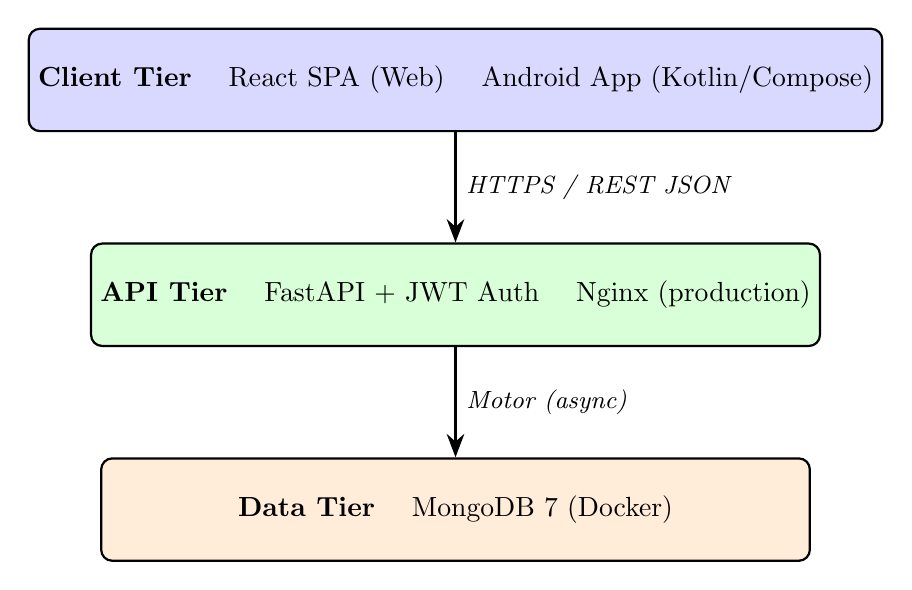
\begin{tikzpicture}[
            node distance=1.4cm,
            box/.style={rectangle, draw=black, thick, minimum width=9cm, minimum height=1.3cm,
                    text centered, rounded corners=4pt, font=\normalsize},
            clientbox/.style={box, fill=blue!15},
            apibox/.style={box, fill=green!15},
            databox/.style={box, fill=orange!15},
            arrow/.style={-Stealth, thick, line width=1.2pt}
        ]
        \node[clientbox] (client) {
            \textbf{Client Tier}~~~
            React SPA (Web) \quad Android App (Kotlin/Compose)
        };
        \node[apibox, below=of client] (api) {
            \textbf{API Tier}~~~
            FastAPI + JWT Auth \quad Nginx (production)
        };
        \node[databox, below=of api] (data) {
            \textbf{Data Tier}~~~
            MongoDB 7 (Docker)
        };
        \draw[arrow] (client) -- node[right, font=\small\itshape]{HTTPS / REST JSON} (api);
        \draw[arrow] (api) -- node[right, font=\small\itshape]{Motor (async)} (data);
    \end{tikzpicture}
    \caption{Three-Tier System Architecture}
    \label{fig:architecture}
\end{figure}

\subsection{Design Principles}

\begin{itemize}
    \item \textbf{RESTful API:} Standard HTTP methods and resource-based URLs with JSON responses
    \item \textbf{Service layer pattern:} Business logic in service classes, separated from API route handlers
    \item \textbf{Component-based frontend:} Modular React components organized by domain
    \item \textbf{Async throughout:} FastAPI async endpoints with async Motor database driver
\end{itemize}

\section{UML Diagrams}

\subsection{Use Case Diagram}

Figure~\ref{fig:usecase} shows the three actor roles and their system use cases. Moderator inherits all Regular User use cases and adds content moderation. Admin inherits all Moderator use cases and adds user governance.

\begin{figure}[p]
    \centering
    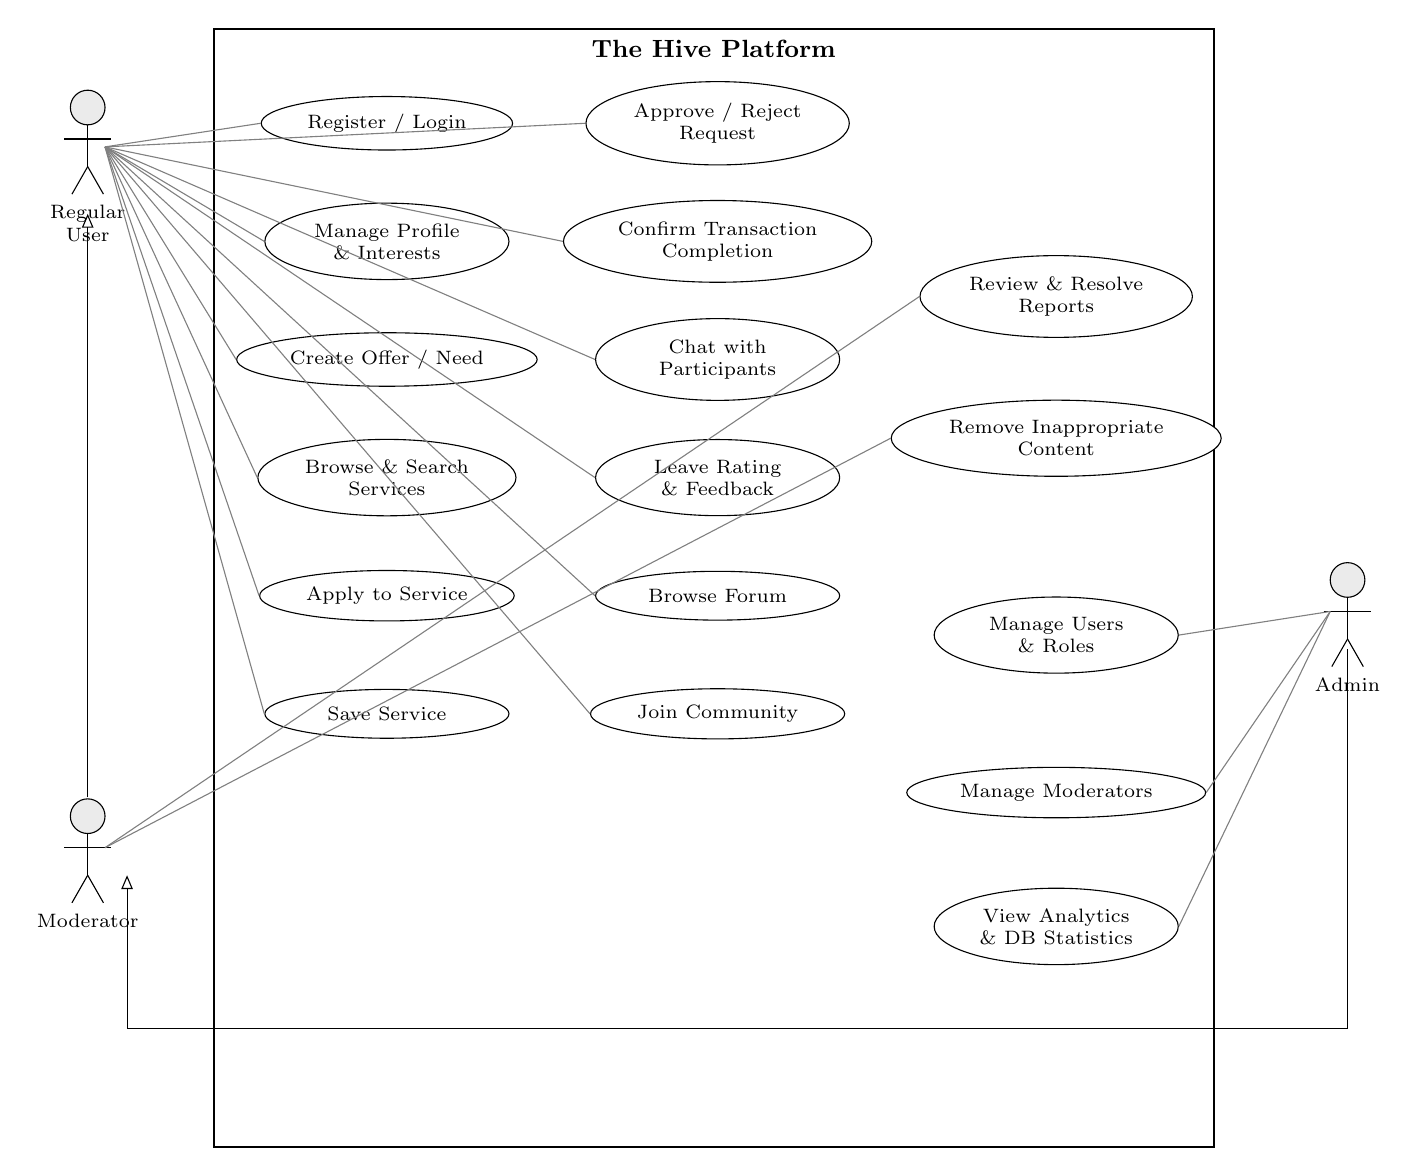
\begin{tikzpicture}[
        uc/.style={ellipse, draw, align=center, font=\scriptsize,
                minimum width=3.1cm, minimum height=0.62cm, fill=white},
        gen/.style={draw, -{Triangle[open,length=5pt]}}
        ]
        \draw[thick] (0.8, 1.2) rectangle (13.5, -13.0);
        \node[font=\small\bfseries] at (7.15, 0.95) {\textsc{The Hive Platform}};

        \node[uc] (uc1)  at (3,  0)    {Register / Login};
        \node[uc] (uc2)  at (3, -1.5)  {Manage Profile\\\& Interests};
        \node[uc] (uc3)  at (3, -3.0)  {Create Offer / Need};
        \node[uc] (uc4)  at (3, -4.5)  {Browse \& Search\\Services};
        \node[uc] (uc5)  at (3, -6.0)  {Apply to Service};
        \node[uc] (uc6)  at (3, -7.5)  {Save Service};

        \node[uc] (uc7)  at (7.2,  0)   {Approve / Reject\\Request};
        \node[uc] (uc8)  at (7.2, -1.5) {Confirm Transaction\\Completion};
        \node[uc] (uc9)  at (7.2, -3.0) {Chat with\\Participants};
        \node[uc] (uc10) at (7.2, -4.5) {Leave Rating\\\& Feedback};
        \node[uc] (uc11) at (7.2, -6.0) {Browse Forum};
        \node[uc] (uc12) at (7.2, -7.5) {Join Community};

        \node[uc] (uc13) at (11.5, -2.2) {Review \& Resolve\\Reports};
        \node[uc] (uc14) at (11.5, -4.0) {Remove Inappropriate\\Content};
        \node[uc] (uc15) at (11.5, -6.5) {Manage Users\\\& Roles};
        \node[uc] (uc16) at (11.5, -8.5) {Manage Moderators};
        \node[uc] (uc17) at (11.5,-10.2) {View Analytics\\\& DB Statistics};

        % Regular User
        \draw[fill=black!8] (-0.8, 0.2) circle (0.22cm);
        \draw (-0.8,-0.02)--(-0.8,-0.55); \draw (-1.1,-0.2)--(-0.5,-0.2);
        \draw (-0.8,-0.55)--(-1.0,-0.9); \draw (-0.8,-0.55)--(-0.6,-0.9);
        \node[below,font=\scriptsize,align=center] at (-0.8,-0.92) {Regular\\User};

        % Moderator
        \draw[fill=black!8] (-0.8,-8.8) circle (0.22cm);
        \draw (-0.8,-9.02)--(-0.8,-9.55); \draw (-1.1,-9.2)--(-0.5,-9.2);
        \draw (-0.8,-9.55)--(-1.0,-9.9); \draw (-0.8,-9.55)--(-0.6,-9.9);
        \node[below,font=\scriptsize,align=center] at (-0.8,-9.92) {Moderator};

        % Admin
        \draw[fill=black!8] (15.2,-5.8) circle (0.22cm);
        \draw (15.2,-6.02)--(15.2,-6.55); \draw (14.9,-6.2)--(15.5,-6.2);
        \draw (15.2,-6.55)--(15.0,-6.9); \draw (15.2,-6.55)--(15.4,-6.9);
        \node[below,font=\scriptsize,align=center] at (15.2,-6.92) {Admin};

        % Generalization: Moderator <- Regular User
        \draw[gen] (-0.8,-8.56) -- (-0.8,-1.15);
        % Generalization: Admin <- Moderator (via bottom path)
        \draw[gen] (15.2,-6.68) -- (15.2,-11.5) -- (-0.3,-11.5) -- (-0.3,-9.55);

        % Regular User -> col1 and col2 use cases
        \foreach \uc in {uc1,uc2,uc3,uc4,uc5,uc6,uc7,uc8,uc9,uc10,uc11,uc12} {
                \draw[thin,gray] (-0.58,-0.3) -- (\uc.west);
            }
        % Moderator -> col3 top two
        \draw[thin,gray] (-0.58,-9.2) -- (uc13.west);
        \draw[thin,gray] (-0.58,-9.2) -- (uc14.west);
        % Admin -> col3 bottom three
        \draw[thin,gray] (14.98,-6.2) -- (uc15.east);
        \draw[thin,gray] (14.98,-6.2) -- (uc16.east);
        \draw[thin,gray] (14.98,-6.2) -- (uc17.east);
    \end{tikzpicture}
    \caption{Use Case Diagram --- The Hive Platform}
    \label{fig:usecase}
\end{figure}

\subsection{Class Diagram}

Figure~\ref{fig:classdiagram} shows the nine core domain entities and their relationships.

\begin{figure}[p]
    \centering
    \resizebox{\textwidth}{!}{%
        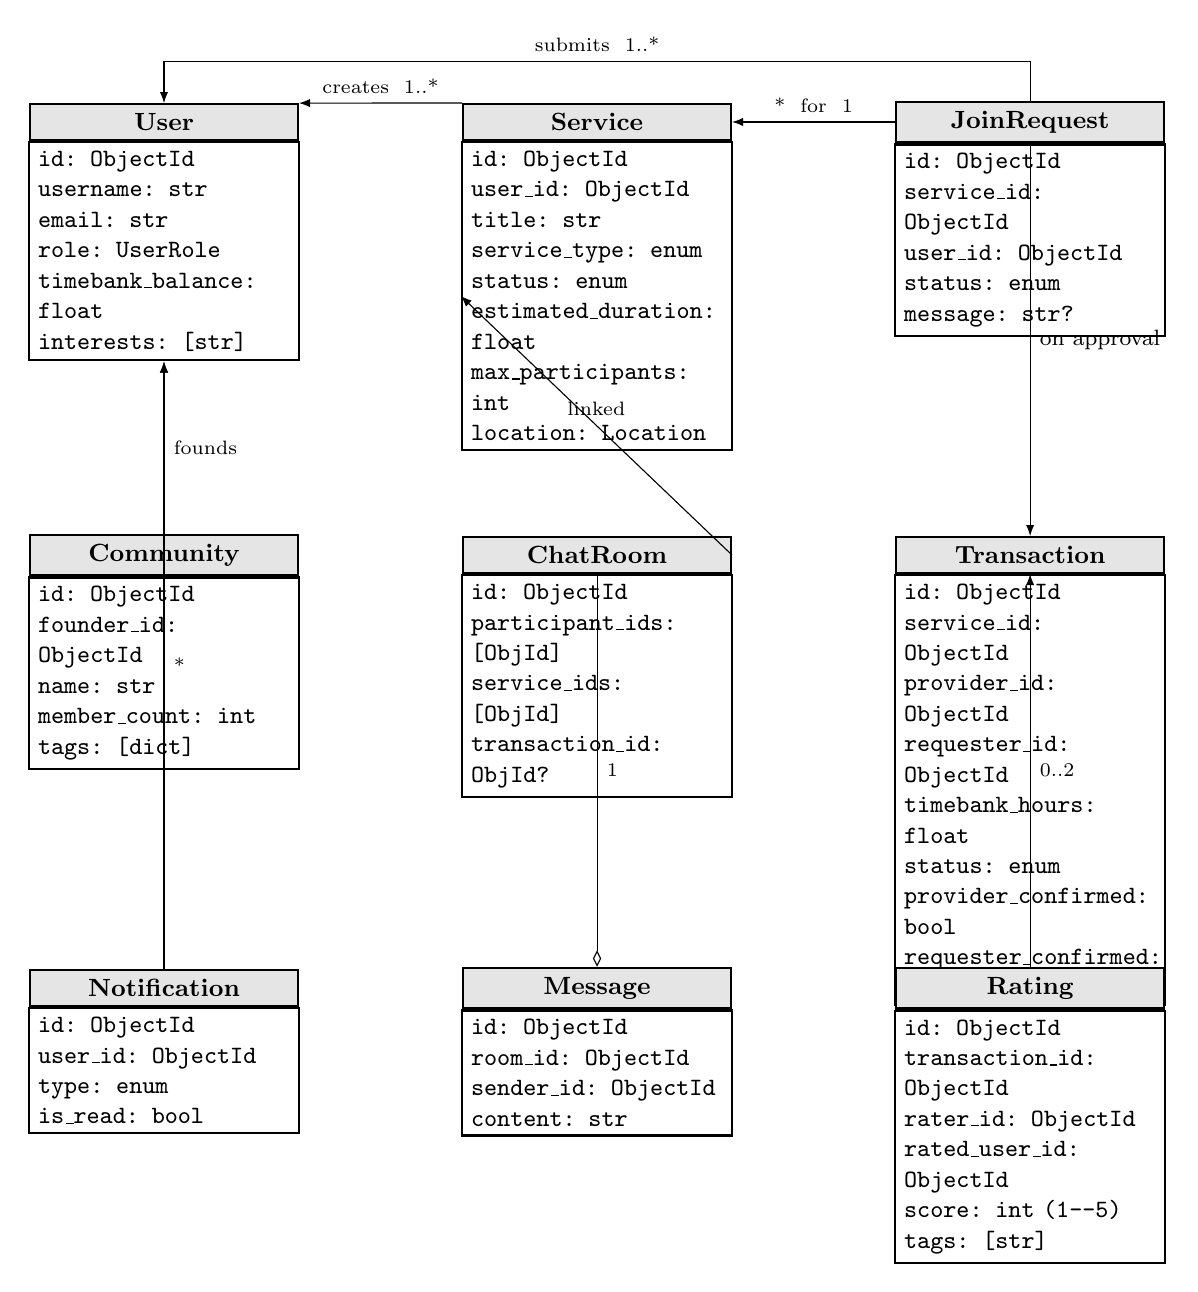
\begin{tikzpicture}[
            cls/.style={rectangle, draw, thick, fill=white,
                    minimum width=3.4cm, font=\small},
            hdr/.style={rectangle, draw, thick, fill=gray!20,
                    minimum width=3.4cm, font=\small\bfseries,
                    align=center},
            rel/.style={draw, -{Latex[length=4pt]}},
            comp/.style={draw, -{Diamond[open,length=6pt]}}
            ]

            %% ---- Entity macros ----
            %% User (0,0)
            \node[hdr] (uhdr) at (0,0)              {User};
            \node[cls, below=0pt of uhdr, align=left, text width=3.2cm] (ubody) {
            \texttt{id: ObjectId}\\
            \texttt{username: str}\\
            \texttt{email: str}\\
            \texttt{role: UserRole}\\
            \texttt{timebank\_balance: float}\\
            \texttt{interests: [str]}
            };

            %% Service (5.5,0)
            \node[hdr] (shdr) at (5.5,0)            {Service};
            \node[cls, below=0pt of shdr, align=left, text width=3.2cm] (sbody) {
                \texttt{id: ObjectId}\\
                \texttt{user\_id: ObjectId}\\
                \texttt{title: str}\\
                \texttt{service\_type: enum}\\
                \texttt{status: enum}\\
                \texttt{estimated\_duration: float}\\
                \texttt{max\_participants: int}\\
                \texttt{location: Location}
            };

            %% JoinRequest (11,0)
            \node[hdr] (jhdr) at (11,0)             {JoinRequest};
            \node[cls, below=0pt of jhdr, align=left, text width=3.2cm] (jbody) {
                \texttt{id: ObjectId}\\
                \texttt{service\_id: ObjectId}\\
                \texttt{user\_id: ObjectId}\\
                \texttt{status: enum}\\
                \texttt{message: str?}
            };

            %% Transaction (11,-5.5)
            \node[hdr] (thdr) at (11,-5.5)          {Transaction};
            \node[cls, below=0pt of thdr, align=left, text width=3.2cm] (tbody) {
                \texttt{id: ObjectId}\\
                \texttt{service\_id: ObjectId}\\
                \texttt{provider\_id: ObjectId}\\
                \texttt{requester\_id: ObjectId}\\
                \texttt{timebank\_hours: float}\\
                \texttt{status: enum}\\
                \texttt{provider\_confirmed: bool}\\
                \texttt{requester\_confirmed: bool}
            };

            %% Rating (11,-11)
            \node[hdr] (rhdr) at (11,-11)           {Rating};
            \node[cls, below=0pt of rhdr, align=left, text width=3.2cm] (rbody) {
            \texttt{id: ObjectId}\\
            \texttt{transaction\_id: ObjectId}\\
            \texttt{rater\_id: ObjectId}\\
            \texttt{rated\_user\_id: ObjectId}\\
            \texttt{score: int (1--5)}\\
            \texttt{tags: [str]}
            };

            %% ChatRoom (5.5,-5.5)
            \node[hdr] (crhdr) at (5.5,-5.5)        {ChatRoom};
            \node[cls, below=0pt of crhdr, align=left, text width=3.2cm] (crbody) {
                \texttt{id: ObjectId}\\
                \texttt{participant\_ids: [ObjId]}\\
                \texttt{service\_ids: [ObjId]}\\
                \texttt{transaction\_id: ObjId?}
            };

            %% Message (5.5,-11)
            \node[hdr] (mhdr) at (5.5,-11)          {Message};
            \node[cls, below=0pt of mhdr, align=left, text width=3.2cm] (mbody) {
                \texttt{id: ObjectId}\\
                \texttt{room\_id: ObjectId}\\
                \texttt{sender\_id: ObjectId}\\
                \texttt{content: str}
            };

            %% Community (0,-5.5)
            \node[hdr] (cohdr) at (0,-5.5)          {Community};
            \node[cls, below=0pt of cohdr, align=left, text width=3.2cm] (cobody) {
            \texttt{id: ObjectId}\\
            \texttt{founder\_id: ObjectId}\\
            \texttt{name: str}\\
            \texttt{member\_count: int}\\
            \texttt{tags: [dict]}
            };

            %% Notification (0,-11)
            \node[hdr] (nhdr) at (0,-11)            {Notification};
            \node[cls, below=0pt of nhdr, align=left, text width=3.2cm] (nbody) {
                \texttt{id: ObjectId}\\
                \texttt{user\_id: ObjectId}\\
                \texttt{type: enum}\\
                \texttt{is\_read: bool}
            };

            %% ---- Relationships ----
            % User creates Services  (1 to many)
            \draw[rel] (shdr.north west) -- node[above,font=\scriptsize]{creates~~1..*} (uhdr.north east);
            % User submits JoinRequests
            \draw[rel] (jhdr.north) -- ++(0,0.5) -| node[above,font=\scriptsize,pos=0.25]{submits~~1..*} (uhdr.north);
            % Service receives JoinRequests
            \draw[rel] (jhdr.west) -- node[above,font=\scriptsize]{*~~for~~1} (shdr.east);
            % JoinRequest leads to Transaction (on approval)
            \draw[rel] (jhdr.south) -- node[right,font=\scriptsize]{\footnotesize on approval} (thdr.north);
            % Transaction generates Ratings
            \draw[rel] (rhdr.north) -- node[right,font=\scriptsize]{0..2} (thdr.south);
            % Service has ChatRoom
            \draw[rel] (crhdr.east) -- node[above,font=\scriptsize]{linked} (sbody.west);
            % ChatRoom contains Messages
            \draw[comp] (crhdr.south) -- node[right,font=\scriptsize]{1} (mhdr.north);
            % User receives Notifications
            \draw[rel] (nhdr.north) -- node[right,font=\scriptsize]{*} (ubody.south);
            % User founds Community
            \draw[rel] (cohdr.north) -- node[right,font=\scriptsize]{founds} (ubody.south);
        \end{tikzpicture}}
    \caption{Class Diagram --- Core Domain Entities}
    \label{fig:classdiagram}
\end{figure}

\subsection{Sequence Diagram: Service Exchange Flow}

Figure~\ref{fig:sequence} traces the complete service exchange from application through TimeBank credit transfer.

\begin{figure}[p]
    \centering
    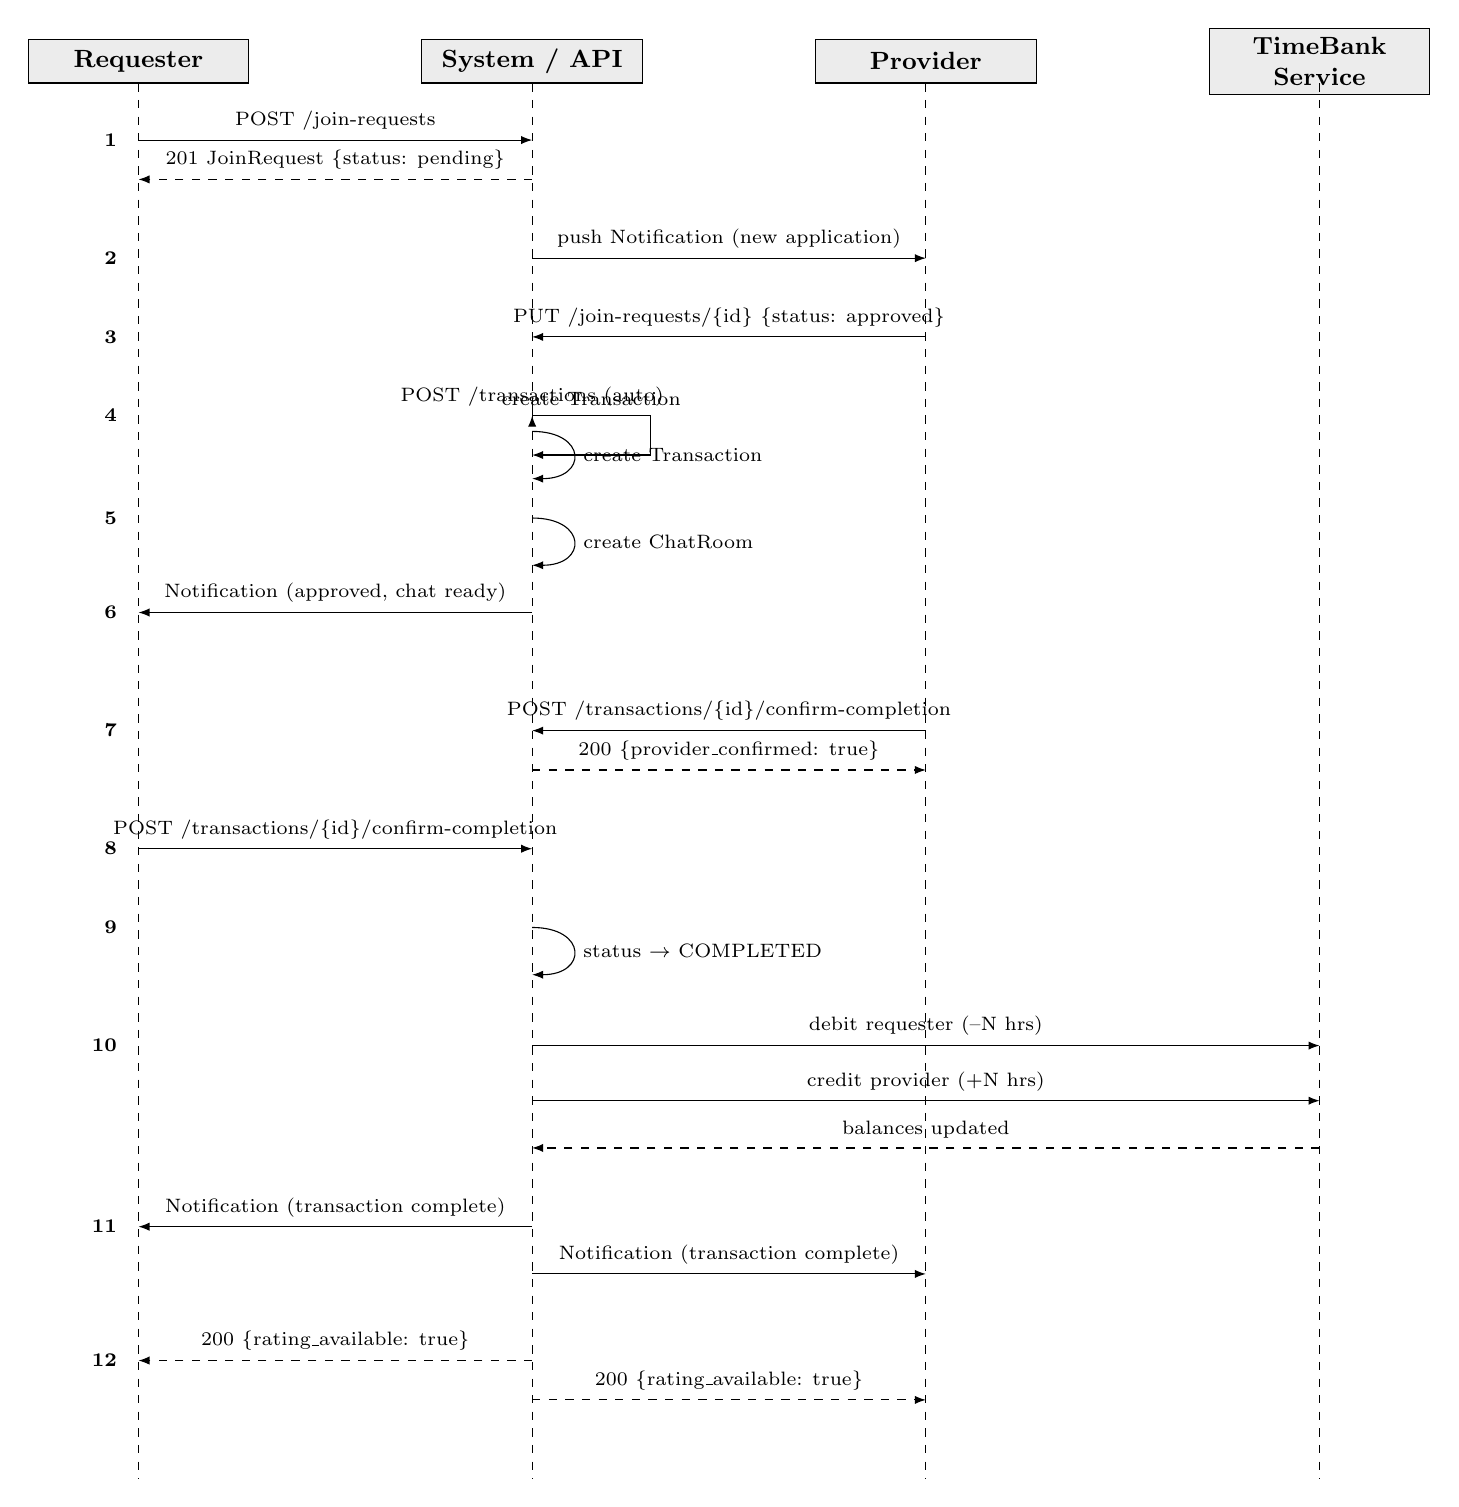
\begin{tikzpicture}[
        lbl/.style={font=\scriptsize, above, sloped=false},
        msg/.style={draw, -{Latex[length=4pt]}, thin},
        ret/.style={draw, -{Latex[length=4pt]}, thin, dashed},
        act/.style={rectangle, draw, fill=white, minimum width=0.25cm}
        ]

        %% Lifeline headers
        \node[draw, fill=gray!15, minimum width=2.8cm, minimum height=0.55cm,
            font=\small\bfseries, align=center] (R) at (0,0)    {Requester};
        \node[draw, fill=gray!15, minimum width=2.8cm, minimum height=0.55cm,
            font=\small\bfseries, align=center] (S) at (5,0)    {System / API};
        \node[draw, fill=gray!15, minimum width=2.8cm, minimum height=0.55cm,
            font=\small\bfseries, align=center] (P) at (10,0)   {Provider};
        \node[draw, fill=gray!15, minimum width=2.8cm, minimum height=0.55cm,
            font=\small\bfseries, align=center] (T) at (15,0)   {TimeBank\\Service};

        %% Lifelines (dashed vertical)
        \draw[dashed,thin] (0,-0.28)  -- (0,-18);
        \draw[dashed,thin] (5,-0.28)  -- (5,-18);
        \draw[dashed,thin] (10,-0.28) -- (10,-18);
        \draw[dashed,thin] (15,-0.28) -- (15,-18);

        %% ---- Step 1: Apply ----
        \node[font=\scriptsize, left] at (-0.15,-1) {\textbf{1}};
        \draw[msg] (0,-1) -- node[lbl]{POST /join-requests} (5,-1);
        \draw[ret] (5,-1.5) -- node[lbl]{201 JoinRequest \{status: pending\}} (0,-1.5);

        %% ---- Step 2: Notify Provider ----
        \node[font=\scriptsize, left] at (-0.15,-2.5) {\textbf{2}};
        \draw[msg] (5,-2.5) -- node[lbl]{push Notification (new application)} (10,-2.5);

        %% ---- Step 3: Approve ----
        \node[font=\scriptsize, left] at (-0.15,-3.5) {\textbf{3}};
        \draw[msg] (10,-3.5) -- node[lbl]{PUT /join-requests/\{id\} \{status: approved\}} (5,-3.5);

        %% ---- Step 4: Create Transaction ----
        \node[font=\scriptsize, left] at (-0.15,-4.5) {\textbf{4}};
        \draw[msg] (5,-4.5) -- node[lbl,above]{POST /transactions (auto)} (5,-4.5);
        \draw[msg] (5,-4.5) -- ++(1.5,0) -- ++(0,-0.5) -- ++(-1.5,0);
        \node[font=\scriptsize, above] at (5.75,-4.5) {create Transaction};

        %% Redraw step 4 more cleanly as a self-message
        \draw[msg] (5,-4.7) to[out=0,in=0,looseness=3] node[right,font=\scriptsize]{create Transaction} (5,-5.3);

        %% ---- Step 5: Create ChatRoom ----
        \node[font=\scriptsize, left] at (-0.15,-5.8) {\textbf{5}};
        \draw[msg] (5,-5.8) to[out=0,in=0,looseness=3] node[right,font=\scriptsize]{create ChatRoom} (5,-6.4);

        %% ---- Step 6: Notify Requester ----
        \node[font=\scriptsize, left] at (-0.15,-7) {\textbf{6}};
        \draw[msg] (5,-7) -- node[lbl]{Notification (approved, chat ready)} (0,-7);

        %% ---- Step 7: Provider confirms completion ----
        \node[font=\scriptsize, left] at (-0.15,-8.5) {\textbf{7}};
        \draw[msg] (10,-8.5) -- node[lbl]{POST /transactions/\{id\}/confirm-completion} (5,-8.5);
        \draw[ret] (5,-9) -- node[lbl]{200 \{provider\_confirmed: true\}} (10,-9);

        %% ---- Step 8: Requester confirms completion ----
        \node[font=\scriptsize, left] at (-0.15,-10) {\textbf{8}};
        \draw[msg] (0,-10) -- node[lbl]{POST /transactions/\{id\}/confirm-completion} (5,-10);

        %% ---- Step 9: Finalize transaction ----
        \node[font=\scriptsize, left] at (-0.15,-11) {\textbf{9}};
        \draw[msg] (5,-11) to[out=0,in=0,looseness=3] node[right,font=\scriptsize]{status $\to$ COMPLETED} (5,-11.6);

        %% ---- Step 10: Update TimeBank ----
        \node[font=\scriptsize, left] at (-0.15,-12.5) {\textbf{10}};
        \draw[msg] (5,-12.5) -- node[lbl]{debit requester (--N hrs)} (15,-12.5);
        \draw[msg] (5,-13.2) -- node[lbl]{credit provider (+N hrs)} (15,-13.2);
        \draw[ret] (15,-13.8) -- node[lbl]{balances updated} (5,-13.8);

        %% ---- Step 11: Notify both parties ----
        \node[font=\scriptsize, left] at (-0.15,-14.8) {\textbf{11}};
        \draw[msg] (5,-14.8) -- node[lbl]{Notification (transaction complete)} (0,-14.8);
        \draw[msg] (5,-15.4) -- node[lbl]{Notification (transaction complete)} (10,-15.4);

        %% ---- Step 12: Rating unlocked ----
        \node[font=\scriptsize, left] at (-0.15,-16.5) {\textbf{12}};
        \draw[ret] (5,-16.5) -- node[lbl]{200 \{rating\_available: true\}} (0,-16.5);
        \draw[ret] (5,-17)   -- node[lbl]{200 \{rating\_available: true\}} (10,-17);

    \end{tikzpicture}
    \caption{Sequence Diagram --- Service Exchange and TimeBank Transfer}
    \label{fig:sequence}
\end{figure}

\section{Scenarios and Mockups}

UI mockups and user scenarios produced during the design phase are available at:
\begin{center}
    \url{https://github.com/senaoz/SWE-574/wiki/Scenarios-\&-Mockups}
\end{center}

Key screens that were mockup'd and implemented:
\begin{itemize}
    \item \textbf{Home page:} Hero section, community values, recent services preview, interactive map
    \item \textbf{Dashboard:} Service grid + map side-by-side, search bar, filters
    \item \textbf{Service Detail:} Full info card, provider profile, location map, apply/chat/save buttons, comments
    \item \textbf{Profile:} Tabs for Services, Applications, Transactions, TimeBank; badge display; ratings
    \item \textbf{Forum:} Discussions/Events tabs; community spaces
    \item \textbf{Admin Panel:} User management, service moderation, analytics
\end{itemize}

\section{Database Design}

\subsection{Collections}

\begin{table}[h]
    \centering
    \begin{tabularx}{\textwidth}{|l|X|}
        \hline
        \textbf{Collection}             & \textbf{Purpose}                                  \\
        \hline
        \texttt{users}                  & User accounts, profiles, and settings             \\
        \hline
        \texttt{services}               & Service offers and needs with geolocation         \\
        \hline
        \texttt{join\_requests}         & Applications from users to services               \\
        \hline
        \texttt{transactions}           & Service exchange transactions (dual-confirmation) \\
        \hline
        \texttt{timebank\_transactions} & TimeBank credit audit log                         \\
        \hline
        \texttt{chat\_rooms}            & Chat room metadata and participant lists          \\
        \hline
        \texttt{messages}               & Individual chat messages                          \\
        \hline
        \texttt{saved\_services}        & User bookmarks of services                        \\
        \hline
        \texttt{forum\_discussions}     & Forum discussion topics                           \\
        \hline
        \texttt{forum\_events}          & Forum event announcements                         \\
        \hline
        \texttt{forum\_comments}        & Comments on discussions and events                \\
        \hline
        \texttt{communities}            & Community groups and membership                   \\
        \hline
        \texttt{ratings}                & Post-exchange star ratings and feedback labels    \\
        \hline
        \texttt{reports}                & User-submitted content reports for moderation     \\
        \hline
        \texttt{notifications}          & In-app notifications (also streamed via SSE)      \\
        \hline
    \end{tabularx}
    \caption{MongoDB Collections}
\end{table}

\subsection{Key Indexes}

\begin{itemize}
    \item \textbf{Unique:} \texttt{users.email}, \texttt{users.username}
    \item \textbf{Geospatial (2dsphere):} \texttt{services.location} (GeoJSON Point format: \texttt{[longitude, latitude]})
    \item \textbf{Compound unique:} \texttt{saved\_services(user\_id, service\_id)}
    \item \textbf{Partial unique:} \texttt{reports(reported\_by, report\_type, reported\_id)} where \texttt{status = ``pending''}
    \item Standard indexes on \texttt{user\_id}, \texttt{service\_id}, \texttt{status}, \texttt{created\_at} across most collections
\end{itemize}

\section{API Design}

\subsection{RESTful Principles}

\begin{itemize}
    \item Resource-based URLs with standard HTTP methods (GET, POST, PUT, DELETE)
    \item JSON request and response bodies
    \item Standard HTTP status codes
    \item JWT Bearer token authentication on protected routes
\end{itemize}

\subsection{Standard Response Envelope}

\begin{lstlisting}
{
  "data": { ... },
  "message": "Success",
  "status": "success"
}
\end{lstlisting}

\subsection{Authentication}

All protected endpoints require: \texttt{Authorization: Bearer <jwt\_token>}

Token properties: HS256 algorithm, 30-minute expiry, subject = user ID.

Full interactive API documentation: \url{https://backend-swe.gnahh5.easypanel.host/docs}

\section{Frontend Architecture}

\subsection{Routing}

\begin{table}[h]
    \centering
    \begin{tabularx}{\textwidth}{|l|X|}
        \hline
        \textbf{Route}                                & \textbf{Access}      \\
        \hline
        \texttt{/}                                    & Public               \\
        \hline
        \texttt{/register}                            & Guest only           \\
        \hline
        \texttt{/dashboard}                           & Authenticated user   \\
        \hline
        \texttt{/service/:id}                         & Authenticated user   \\
        \hline
        \texttt{/user/:userId}                        & Authenticated user   \\
        \hline
        \texttt{/profile}                             & Authenticated user   \\
        \hline
        \texttt{/forum}                               & Authenticated user   \\
        \hline
        \texttt{/forum/discussions/:id}               & Authenticated user   \\
        \hline
        \texttt{/forum/events/:id}                    & Authenticated user   \\
        \hline
        \texttt{/forum/communities/:id}               & Authenticated user   \\
        \hline
        \texttt{/forum/communities/:id/posts/:postId} & Authenticated user   \\
        \hline
        \texttt{/settings}                            & Authenticated user   \\
        \hline
        \texttt{/admin}                               & Moderator/Admin only \\
        \hline
    \end{tabularx}
    \caption{Frontend Routes}
\end{table}

\subsection{State Management}

\begin{itemize}
    \item \textbf{React Query:} Server state (all API calls, caching, invalidation)
    \item \textbf{UserContext:} Current user, auth token presence, refetch trigger
    \item \textbf{FilterContext:} Global service search/filter state
    \item \textbf{ThemeContext:} Dark/light mode toggle (persisted to localStorage)
    \item \textbf{localStorage:} JWT access token, theme preference
\end{itemize}

\section{Backend Architecture}

\subsection{Layer Structure}

\begin{itemize}
    \item \textbf{\texttt{api/}:} 15 route handler files --- thin layer delegating to services
    \item \textbf{\texttt{services/}:} Business logic layer --- one class per domain (auth, user, service, transaction, join\_request, chat, comment, forum, community, rating, report, notification, badge, wikidata, content\_moderation)
    \item \textbf{\texttt{models/}:} Pydantic schemas for request/response validation
    \item \textbf{\texttt{core/}:} \texttt{config.py} (settings), \texttt{database.py} (Motor + index creation), \texttt{security.py} (JWT/bcrypt), \texttt{permissions.py} (RBAC)
\end{itemize}

\subsection{RBAC}

Roles: \texttt{user}, \texttt{moderator}, \texttt{admin}, \texttt{banned}.

Dependency functions in \texttt{core/permissions.py}:
\begin{itemize}
    \item \texttt{require\_role([roles])} --- generic role check
    \item \texttt{require\_moderator\_or\_admin()} --- for admin/moderation routes
    \item \texttt{require\_any\_role()} --- any authenticated user
\end{itemize}

% =========================================================
\chapter{Requirement Completion Status}
% =========================================================

\section{Summary}

\begin{table}[h]
    \centering
    \begin{tabularx}{\textwidth}{|l|X|X|}
        \hline
        \textbf{Category}             & \textbf{Total} & \textbf{Status}     \\
        \hline
        Functional Requirement Groups & 19             & 19 complete (100\%) \\
        \hline
        Non-Functional Requirements   & 15             & 13 complete (87\%)  \\
        \hline
        \textbf{Overall}              & \textbf{34}    & \textbf{32 (94\%)}  \\
        \hline
    \end{tabularx}
    \caption{Requirement Completion Summary}
\end{table}

Partially completed:
\begin{itemize}
    \item \textbf{NFR--1 (500+ concurrent users):} Architecture supports scaling but load testing not performed.
    \item \textbf{NFR--10 (Daily DB backups):} Manual procedures documented; not automated.
\end{itemize}

\section{Detailed Status}

\begin{longtable}{|p{5.5cm}|p{2cm}|p{6cm}|}
    \hline
    \textbf{Requirement}              & \textbf{Status} & \textbf{Notes}                                        \\
    \hline
    \endhead
    FR--1: Authentication             & Complete        & JWT, bcrypt, interest selection on register           \\
    \hline
    FR--2: Profile Management         & Complete        & Tags, bio, profile picture, interests                 \\
    \hline
    FR--3: Offer/Need Management      & Complete        & Full CRUD, capacity, tags, location                   \\
    \hline
    FR--4: Availability               & Complete        & Duration-based scheduling                             \\
    \hline
    FR--5: Handshake Mechanism        & Complete        & Join request workflow with full state machine         \\
    \hline
    FR--6: Messaging System           & Complete        & Chat rooms auto-created on approval                   \\
    \hline
    FR--7: TimeBank System            & Complete        & Whole-hour, 10-hour cap, anti-hoarding rule           \\
    \hline
    FR--8: Tagging and Search         & Complete        & Wikidata integration, active-tag filtering            \\
    \hline
    FR--9: Map Visualization          & Complete        & Google Maps, fuzzed locations, type differentiation   \\
    \hline
    FR--10: Comment and Feedback      & Complete        & Ratings, labels, images, content moderation           \\
    \hline
    FR--11: Reporting and Moderation  & Complete        & Report submission, moderator review, audit log        \\
    \hline
    FR--12: Completion/Transparency   & Complete        & Exchange history on profile                           \\
    \hline
    FR--13: Badges                    & Complete        & 12 badge types, auto-awarded, dynamic recalculation   \\
    \hline
    FR--14: Active Items Management   & Complete        & Profile tabs for services, applications, transactions \\
    \hline
    FR--15: Community Forum           & Complete        & Discussions, Events, upvotes, comments, pinning       \\
    \hline
    FR--16: User Interaction Features & Complete        & Save services, share URL                              \\
    \hline
    FR--17: Mobile-Specific Features  & Complete        & Android app; offline queue, deep links, share sheet   \\
    \hline
    FR--18: Recommendations           & Complete        & Tag-based + proximity scoring                         \\
    \hline
    FR--19: Communities               & Complete        & Creation, join, posts, events, member management      \\
    \hline
    NFR--1: 500+ concurrent users     & Partial         & Architecture supports it; not load-tested             \\
    \hline
    NFR--10: Daily DB backups         & Partial         & Procedures documented; not automated                  \\
    \hline
\end{longtable}

% =========================================================
\chapter{System Manual}
% =========================================================

\section{Runtime Requirements}

\subsection{Minimum Requirements}

\begin{itemize}
    \item Docker 20.10+ and Docker Compose 2.0+
    \item 2 GB RAM minimum (4 GB recommended)
    \item 10 GB available disk space
    \item Internet connection (Google Maps API, Wikidata API)
\end{itemize}

\subsection{Production Requirements}

\begin{itemize}
    \item VPS with at least 2 GB RAM
    \item MongoDB 7 (managed or containerized)
    \item Domain name with SSL certificate (HTTPS required)
    \item Google Maps API key
\end{itemize}

\section{Docker Setup}

\subsection{Container Architecture}

Docker Compose orchestrates three containers:

\begin{enumerate}
    \item \textbf{frontend:} React SPA (Vite build) served by Nginx on port 80
    \item \textbf{backend:} FastAPI (Uvicorn) on port 8000
    \item \textbf{mongodb:} MongoDB 7, port 38017 (mapped from internal 27017)
\end{enumerate}

Key files: \texttt{docker-compose.yml}, \texttt{backend/Dockerfile}, \texttt{frontend/Dockerfile}.

\section{Installation Instructions}

\subsection{Quick Start with Docker}

\begin{enumerate}
    \item Clone the repository:
          \begin{lstlisting}[language=bash]
git clone <https://github.com/senaoz/SWE-574.git>
cd SWE-574
    \end{lstlisting}

    \item Create environment files:
          \begin{lstlisting}[language=bash]
cp backend/.env.example backend/.env
cp frontend/.env.example frontend/.env
    \end{lstlisting}

    \item Edit the \texttt{.env} files with your configuration

    \item Build and start all services:
          \begin{lstlisting}[language=bash]
docker compose up -d --build
    \end{lstlisting}

    \item Access the application:
          \begin{itemize}
              \item Frontend: \url{http://localhost}
              \item Backend API: \url{http://localhost:8000}
              \item API Documentation: \url{http://localhost:8000/docs}
          \end{itemize}
\end{enumerate}

\subsection{Local Backend Development (without Docker)}

Must be run from the \texttt{backend/} directory (relative imports break if run from the project root):

\begin{lstlisting}[language=bash]
cd backend
pip install -r requirements.txt
uvicorn app.main:app --reload --host 0.0.0.0 --port 8000
\end{lstlisting}

\subsection{Local Frontend Development}

\begin{lstlisting}[language=bash]
cd frontend
npm install
npm run dev          # Dev server on port 3000
npm run build        # Production build
npm run type-check   # TypeScript validation
npm test             # Vitest unit tests
\end{lstlisting}

\section{Environment Variables}

\subsection{Backend (\texttt{backend/.env})}

\begin{table}[h]
    \centering
    \begin{tabularx}{\textwidth}{|l|X|}
        \hline
        \textbf{Variable}         & \textbf{Description}                           \\
        \hline
        \texttt{MONGODB\_URL}     & MongoDB connection string                      \\
        \hline
        \texttt{DATABASE\_NAME}   & Database name                                  \\
        \hline
        \texttt{SECRET\_KEY}      & JWT secret key                                 \\
        \hline
        \texttt{ALLOWED\_ORIGINS} & CORS allowed origins (comma-separated)         \\
        \hline
        \texttt{DEBUG}            & Debug mode flag (\texttt{true}/\texttt{false}) \\
        \hline
    \end{tabularx}
    \caption{Backend Environment Variables}
\end{table}

\subsection{Frontend (\texttt{frontend/.env})}

\begin{table}[h]
    \centering
    \begin{tabularx}{\textwidth}{|l|X|}
        \hline
        \textbf{Variable}       & \textbf{Description} \\
        \hline
        \texttt{VITE\_API\_URL} & Backend API base URL \\
        \hline
    \end{tabularx}
    \caption{Frontend Environment Variables}
\end{table}

\section{Production Deployment}

\subsection{CI/CD Pipeline}

Deployment is automated via GitHub Actions (\texttt{.github/workflows/deploy-easypanel.yml}). A push to \texttt{main} triggers a deployment webhook to EasyPanel, which pulls the latest code, builds Docker images, and restarts services.

\subsection{EasyPanel Setup}

\begin{enumerate}
    \item Connect the GitHub repository to EasyPanel
    \item Create three services: Frontend (port 80), Backend (port 8000), and MongoDB (managed)
    \item Set all required environment variables
    \item Configure the deployment webhook secret in GitHub Actions secrets
    \item Deploy and verify via \texttt{GET /health} endpoint
\end{enumerate}

% =========================================================
\chapter{User Manual}
% =========================================================

\section{Getting Started}

Navigate to \url{https://swe.gnahh5.easypanel.host} in any modern web browser.

\subsection{Registration}

\begin{enumerate}
    \item Click \textbf{``Sign Up''} on the home page
    \item Fill in: username (unique), email, password (min 8 characters), confirm password, full name
    \item Select at least one interest tag (used for personalized recommendations)
    \item Submit --- you are logged in automatically
\end{enumerate}

\subsection{Login}

\begin{enumerate}
    \item Click \textbf{``Login''}
    \item Enter your email and password
    \item You are redirected to the dashboard
\end{enumerate}

\section{Key Features}

\subsection{Creating a Service}

\begin{enumerate}
    \item Click \textbf{``Create Service''} in the dashboard
    \item Select: \textbf{Offer} (I can provide this) or \textbf{Need} (I need this)
    \item Fill in: title, description, category, duration (whole hours), location, tags
    \item Submit --- service appears on dashboard and map immediately
\end{enumerate}

\subsection{Discovering Services}

\begin{itemize}
    \item \textbf{Dashboard:} Grid of all active services
    \item \textbf{Search bar:} Keyword search across title, description, and tags
    \item \textbf{Filters:} Narrow by category, city, or service type
    \item \textbf{Interactive map:} Click markers to see service previews
    \item \textbf{Recommendations:} ``Recommended for You'' section based on interests
\end{itemize}

\subsection{Applying to a Service}

\begin{enumerate}
    \item Click on a service card to view details
    \item Click \textbf{``Apply''} and optionally add a message
    \item Your request shows``Pending'' status in Profile \textrightarrow{} Applications
\end{enumerate}

\subsection{Managing Join Requests (as Provider)}

\begin{enumerate}
    \item Go to Profile \textrightarrow{} Services tab, open your service
    \item View the Applicants section and review applicant profiles
    \item Approve or reject each application
    \item On approval: transaction is created automatically; chat room opens
\end{enumerate}

\subsection{Completing Transactions}

Both parties must confirm:

\begin{enumerate}
    \item Go to Profile \textrightarrow{} Transactions tab
    \item Click \textbf{``Confirm Completion''} on the active transaction
    \item When both parties confirm: transaction finalizes, TimeBank balances update, rating form unlocks
\end{enumerate}

\subsection{Using Chat}

\begin{enumerate}
    \item Navigate to the Chat page or click \textbf{``Chat''} on any service detail page
    \item Select a room from the sidebar and type/send messages
    \item Chat rooms are automatically linked to services or transactions
\end{enumerate}

\subsection{TimeBank System}

\begin{itemize}
    \item Starting balance: 3 hours; maximum: 10 hours
    \item Only whole-hour transactions supported
    \item When you reach 10 hours, you must post a Need to earn more
    \item View your balance and full history in Profile \textrightarrow{} TimeBank tab
\end{itemize}

\subsection{Forum and Communities}

\begin{itemize}
    \item \textbf{Forum Discussions:} Create threads, comment, upvote; search by keyword or tag
    \item \textbf{Forum Events:} Announce events with date/time; mark attendance
    \item \textbf{Communities:} Join groups, contribute posts, view unified community feed
\end{itemize}

\subsection{Profile and Badges}

\begin{itemize}
    \item Your profile shows completed exchanges, ratings, interest tags, and earned badges
    \item Badges are awarded automatically (e.g., ``Honey Maker'' for first completed exchange)
    \item Update profile, interests, and profile picture in Settings
\end{itemize}

% =========================================================
\chapter{API Documentation}
% =========================================================

\section{Overview}

The Hive Platform backend exposes a RESTful API. Full interactive documentation (Swagger UI):
\begin{center}
    \url{https://backend-swe.gnahh5.easypanel.host/docs}
\end{center}

\subsection{Authentication}

All protected endpoints require:
\begin{lstlisting}
Authorization: Bearer <access_token>
\end{lstlisting}
Tokens are obtained via \texttt{POST /login}. Expiry: 30 minutes.

\subsection{Response Format}

\begin{lstlisting}
{
  "data": { ... },
  "message": "Success",
  "status": "success"
}
\end{lstlisting}

\section{Endpoint Reference}

\subsection{Authentication}

\begin{longtable}{|l|p{6.5cm}|p{5cm}|l|}
    \hline
    \textbf{Method} & \textbf{Path}      & \textbf{Description}     & \textbf{Auth} \\
    \hline
    \endhead
    POST            & \texttt{/register} & Register a new user      & No            \\
    \hline
    POST            & \texttt{/login}    & Login; returns JWT token & No            \\
    \hline
    GET             & \texttt{/me}       & Get current user info    & Yes           \\
    \hline
\end{longtable}

\subsection{Users}

\begin{longtable}{|l|p{6.5cm}|p{5cm}|l|}
    \hline
    \textbf{Method} & \textbf{Path}                 & \textbf{Description}           & \textbf{Auth} \\
    \hline
    \endhead
    GET             & \texttt{/profile}             & Get own profile                & Yes           \\
    \hline
    PUT             & \texttt{/profile}             & Update own profile             & Yes           \\
    \hline
    GET             & \texttt{/timebank}            & Get TimeBank balance + history & Yes           \\
    \hline
    GET             & \texttt{/badges}              & Get own badges                 & Yes           \\
    \hline
    GET             & \texttt{/settings}            & Get user settings              & Yes           \\
    \hline
    PUT             & \texttt{/settings}            & Update user settings           & Yes           \\
    \hline
    POST            & \texttt{/change-password}     & Change password                & Yes           \\
    \hline
    GET             & \texttt{/search}              & Search users                   & Yes           \\
    \hline
    GET             & \texttt{/\{user\_id\}}        & Get public profile by ID       & Yes           \\
    \hline
    GET             & \texttt{/\{user\_id\}/badges} & Get badges for a user          & Yes           \\
    \hline
    PUT             & \texttt{/\{user\_id\}/role}   & Update user role               & Admin         \\
    \hline
\end{longtable}

\subsection{Services}

\begin{longtable}{|l|p{6.5cm}|p{5cm}|l|}
    \hline
    \textbf{Method} & \textbf{Path}                      & \textbf{Description}             & \textbf{Auth} \\
    \hline
    \endhead
    GET             & \texttt{/services}                 & List/search services             & Yes           \\
    \hline
    POST            & \texttt{/services}                 & Create a service                 & Yes           \\
    \hline
    GET             & \texttt{/services/saved}           & Get saved services               & Yes           \\
    \hline
    GET             & \texttt{/services/recommendations} & Get personalized recommendations & Yes           \\
    \hline
    GET             & \texttt{/services/\{id\}}          & Get service details              & Yes           \\
    \hline
    PUT             & \texttt{/services/\{id\}}          & Update a service                 & Yes           \\
    \hline
    DELETE          & \texttt{/services/\{id\}}          & Delete a service                 & Yes           \\
    \hline
    POST            & \texttt{/services/\{id\}/save}     & Save a service                   & Yes           \\
    \hline
    POST            & \texttt{/services/\{id\}/complete} & Mark service complete            & Yes           \\
    \hline
    POST            & \texttt{/services/\{id\}/cancel}   & Cancel a service                 & Yes           \\
    \hline
\end{longtable}

\subsection{Join Requests}

\begin{longtable}{|l|p{6.5cm}|p{5cm}|l|}
    \hline
    \textbf{Method} & \textbf{Path}                          & \textbf{Description}        & \textbf{Auth} \\
    \hline
    \endhead
    POST            & \texttt{/join-requests}                & Apply to a service          & Yes           \\
    \hline
    GET             & \texttt{/join-requests/my-requests}    & Get own join requests       & Yes           \\
    \hline
    GET             & \texttt{/join-requests/service/\{id\}} & List requests for a service & Yes           \\
    \hline
    PUT             & \texttt{/join-requests/\{id\}}         & Approve or reject a request & Yes           \\
    \hline
    POST            & \texttt{/join-requests/\{id\}/cancel}  & Cancel own pending request  & Yes           \\
    \hline
\end{longtable}

\subsection{Transactions}

\begin{longtable}{|l|p{6.5cm}|p{5cm}|l|}
    \hline
    \textbf{Method} & \textbf{Path}                                    & \textbf{Description}         & \textbf{Auth} \\
    \hline
    \endhead
    POST            & \texttt{/transactions}                           & Create a transaction         & Yes           \\
    \hline
    GET             & \texttt{/transactions/my-transactions}           & Get own transactions         & Yes           \\
    \hline
    POST            & \texttt{/transactions/\{id\}/confirm-completion} & Confirm transaction complete & Yes           \\
    \hline
    GET             & \texttt{/transactions/\{id\}}                    & Get transaction details      & Yes           \\
    \hline
\end{longtable}

\subsection{Chat}

\begin{longtable}{|l|p{6.5cm}|p{5cm}|l|}
    \hline
    \textbf{Method} & \textbf{Path}                        & \textbf{Description}     & \textbf{Auth} \\
    \hline
    \endhead
    GET             & \texttt{/chat/rooms}                 & List chat rooms          & Yes           \\
    \hline
    POST            & \texttt{/chat/rooms}                 & Create a chat room       & Yes           \\
    \hline
    GET             & \texttt{/chat/rooms/\{id\}}          & Get room details         & Yes           \\
    \hline
    GET             & \texttt{/chat/rooms/\{id\}/messages} & Get room message history & Yes           \\
    \hline
    POST            & \texttt{/chat/messages}              & Send a message           & Yes           \\
    \hline
    DELETE          & \texttt{/chat/messages/\{id\}}       & Delete a message         & Yes           \\
    \hline
\end{longtable}

\subsection{Forum}

\begin{longtable}{|l|p{6.5cm}|p{5cm}|l|}
    \hline
    \textbf{Method} & \textbf{Path}                             & \textbf{Description}      & \textbf{Auth} \\
    \hline
    \endhead
    GET             & \texttt{/forum/discussions}               & List discussions          & Yes           \\
    \hline
    POST            & \texttt{/forum/discussions}               & Create a discussion       & Yes           \\
    \hline
    GET             & \texttt{/forum/discussions/\{id\}}        & Get discussion details    & Yes           \\
    \hline
    PUT             & \texttt{/forum/discussions/\{id\}}        & Update a discussion       & Yes           \\
    \hline
    DELETE          & \texttt{/forum/discussions/\{id\}}        & Delete a discussion       & Yes           \\
    \hline
    POST            & \texttt{/forum/discussions/\{id\}/upvote} & Upvote a discussion       & Yes           \\
    \hline
    GET             & \texttt{/forum/events}                    & List events               & Yes           \\
    \hline
    POST            & \texttt{/forum/events}                    & Create an event           & Yes           \\
    \hline
    POST            & \texttt{/forum/events/\{id\}/attend}      & Mark attendance for event & Yes           \\
    \hline
    POST            & \texttt{/forum/comments}                  & Post a comment            & Yes           \\
    \hline
    POST            & \texttt{/forum/comments/\{id\}/upvote}    & Upvote a comment          & Yes           \\
    \hline
\end{longtable}

\subsection{Communities}

\begin{longtable}{|l|p{6.5cm}|p{5cm}|l|}
    \hline
    \textbf{Method} & \textbf{Path}                                     & \textbf{Description}       & \textbf{Auth} \\
    \hline
    \endhead
    GET             & \texttt{/communities}                             & List communities           & Yes           \\
    \hline
    POST            & \texttt{/communities}                             & Create a community         & Yes           \\
    \hline
    GET             & \texttt{/communities/my}                          & Get my communities         & Yes           \\
    \hline
    GET             & \texttt{/communities/\{id\}}                      & Get community details      & Yes           \\
    \hline
    POST            & \texttt{/communities/\{id\}/join}                 & Join a community           & Yes           \\
    \hline
    DELETE          & \texttt{/communities/\{id\}/leave}                & Leave a community          & Yes           \\
    \hline
    GET             & \texttt{/communities/\{id\}/posts}                & List community posts       & Yes           \\
    \hline
    POST            & \texttt{/communities/\{id\}/posts}                & Create a post in community & Yes           \\
    \hline
    POST            & \texttt{/communities/\{id\}/posts/\{pid\}/upvote} & Upvote a community post    & Yes           \\
    \hline
\end{longtable}

\subsection{Ratings}

\begin{longtable}{|l|p{6.5cm}|p{5cm}|l|}
    \hline
    \textbf{Method} & \textbf{Path}                        & \textbf{Description}        & \textbf{Auth} \\
    \hline
    \endhead
    POST            & \texttt{/ratings}                    & Submit a rating             & Yes           \\
    \hline
    GET             & \texttt{/ratings/user/\{user\_id\}}  & Get ratings for a user      & Yes           \\
    \hline
    GET             & \texttt{/ratings/transaction/\{id\}} & Get ratings for transaction & Yes           \\
    \hline
\end{longtable}

\subsection{Notifications}

\begin{longtable}{|l|p{6.5cm}|p{5cm}|l|}
    \hline
    \textbf{Method} & \textbf{Path}                        & \textbf{Description}           & \textbf{Auth} \\
    \hline
    \endhead
    GET             & \texttt{/notifications/stream}       & SSE stream for live updates    & Yes           \\
    \hline
    GET             & \texttt{/notifications/unread-count} & Get unread notification count  & Yes           \\
    \hline
    GET             & \texttt{/notifications}              & List notifications             & Yes           \\
    \hline
    PUT             & \texttt{/notifications/read-all}     & Mark all notifications as read & Yes           \\
    \hline
    PUT             & \texttt{/notifications/\{id\}/read}  & Mark one notification as read  & Yes           \\
    \hline
\end{longtable}

\subsection{Admin}

\begin{longtable}{|l|p{6.5cm}|p{5cm}|l|}
    \hline
    \textbf{Method} & \textbf{Path}                                   & \textbf{Description}         & \textbf{Auth} \\
    \hline
    \endhead
    GET             & \texttt{/admin/db/stats}                        & Database statistics          & Admin         \\
    \hline
    GET             & \texttt{/admin/failed-transactions}             & Failed TimeBank transactions & Admin         \\
    \hline
    GET             & \texttt{/admin/analytics/service-participation} & Participation analytics      & Admin         \\
    \hline
\end{longtable}

\subsection{File Uploads}

Files are uploaded via \texttt{multipart/form-data} to \texttt{/upload/\{type\}} and served as static files at:
\begin{itemize}
    \item \texttt{/uploads/\{type\}/\{filename\}}.
    \item Supported types: \texttt{profile}, \texttt{services}, \texttt{communities}, \texttt{ratings}, \texttt{comments}, \texttt{forum-events}, \texttt{discussions}.
\end{itemize}


\section{Sample Usage Scenarios}

Four scenarios are presented below demonstrating complex, multi-step API workflows introduced or significantly extended in the final milestone.

% ----------------------------------------------------------
\subsection{Scenario 1: Personalised Service Recommendations}
% ----------------------------------------------------------

\textbf{Endpoint:} \texttt{GET /services/recommendations}

\textbf{Description:} A logged-in user requests personalised service recommendations. The backend ranks services by tag overlap with the user's interests, geographic proximity, and recency, returning each result with a human-readable reason and a relevance score.

\textbf{Request:}
\begin{lstlisting}[language=bash]
curl -s \
  -H "Authorization: Bearer $TOKEN" \
  "https://backend-swe.gnahh5.easypanel.host/services/recommendations?limit=2"
\end{lstlisting}

\textbf{Response:}
\begin{lstlisting}
{
  "items": [
    {
      "service": {
        "title": "Home Cooking / Meal Prep",
        "category": null,
        "tags": [
          { "label": "cooking", "entityId": "11476" },
          { "label": "food",    "entityId": "2095"  }
        ],
        "estimated_duration": 2.0,
        "service_type": "offer",
        "status": "active",
        "_id": "69ac0aa29b15aae8e3174d8b"
      },
      "reason": "Because it's similar to services you saved",
      "score": 4.5367,
      "matched_interests": ["Cooking"]
    },
    {
      "service": {
        "title": "Specialty Coffee Home Brewing Workshop",
        "tags": [
          { "label": "Coffee", "entityId": "Q8486" }
        ],
        "estimated_duration": 2.0,
        "service_type": "offer",
        "status": "active",
        "_id": "69ac0aa29b15aae8e3174e12"
      },
      "reason": "Popular in your neighbourhood",
      "score": 3.8102,
      "matched_interests": ["Cooking"]
    }
  ]
}
\end{lstlisting}

% ----------------------------------------------------------
\subsection{Scenario 2: Semantic Tag Search via Wikidata}
% ----------------------------------------------------------

\textbf{Endpoint:} \texttt{GET /wikidata/search}

\textbf{Description:} A user types a keyword while creating a service. The frontend queries this endpoint, which proxies to the Wikidata search API and returns structured concept entities. The user selects an entity (e.g.\ \texttt{Q6607} for ``guitar'') which is stored as a structured tag on the service, enabling semantic filtering beyond simple keyword matching.

\textbf{Request:}
\begin{lstlisting}[language=bash]
curl -s \
  -H "Authorization: Bearer $TOKEN" \
  "https://backend-swe.gnahh5.easypanel.host/wikidata/search\
?query=guitar+lessons&limit=3"
\end{lstlisting}

\textbf{Response:}
\begin{lstlisting}
{
  "query": "guitar lessons",
  "language": "en",
  "results": [
    {
      "title": "Q136036312",
      "pageId": "129754246",
      "snippet": "Interactive guitar-learning application on iOS.",
      "titleSnippet": "Amped Guitar",
      "timestamp": "2025-09-01T09:16:55Z",
      "url": "https://www.wikidata.org/wiki/Q136036312"
    },
    {
      "title": "Q6607",
      "pageId": "7734",
      "snippet": "fretted string instrument",
      "titleSnippet": "guitar",
      "timestamp": "2026-05-11T13:36:07Z",
      "url": "https://www.wikidata.org/wiki/Q6607"
    }
  ],
  "count": 3
}
\end{lstlisting}

% ----------------------------------------------------------
\subsection{Scenario 3: Forum Event Image Upload}
% ----------------------------------------------------------

\textbf{Endpoint:} \texttt{POST /upload/forum-event-image} then \texttt{POST /forum/events}

\textbf{Description:} A moderator creates a forum event with a banner image. The image is first uploaded as \texttt{multipart/form-data}; the returned URL is then embedded in the event creation payload. This two-step media upload workflow was added in the final milestone.

\textbf{Request — Step 1 (upload image):}
\begin{lstlisting}[language=bash]
curl -s -X POST \
  -H "Authorization: Bearer $TOKEN" \
  -F "file=@banner.jpg" \
  "https://backend-swe.gnahh5.easypanel.host/upload/forum-event-image"
\end{lstlisting}

\textbf{Response — Step 1:}
\begin{lstlisting}
{
  "url": "/uploads/forum-events/68f67f9c_1778401261.webp",
  "filename": "68f67f9c_1778401261.webp"
}
\end{lstlisting}

\textbf{Request — Step 2 (create event with banner):}
\begin{lstlisting}[language=bash]
curl -s -X POST \
  -H "Authorization: Bearer $TOKEN" \
  -H "Content-Type: application/json" \
  -d '{
    "title": "Community Repair Café",
    "description": "Bring broken items and fix them together.",
    "location": "Kadıköy, Istanbul",
    "date": "2026-06-14T10:00:00",
    "banner_image_url": "/uploads/forum-events/68f67f9c_1778401261.webp",
    "community_id": null
  }' \
  "https://backend-swe.gnahh5.easypanel.host/forum/events"
\end{lstlisting}

\textbf{Response — Step 2:}
\begin{lstlisting}
{
  "_id": "6a1f3d22abc44e001b3c8f01",
  "title": "Community Repair Café",
  "description": "Bring broken items and fix them together.",
  "date": "2026-06-14T10:00:00",
  "banner_image_url": "/uploads/forum-events/68f67f9c_1778401261.webp",
  "created_by": "68f67f9c3966e4ce6ebcd0d8",
  "attendees": [],
  "created_at": "2026-05-16T12:00:00"
}
\end{lstlisting}

% ----------------------------------------------------------
\subsection{Scenario 4: Join Request with TimeBank Balance Enforcement}
% ----------------------------------------------------------

\textbf{Endpoint:} \texttt{POST /join-requests/}

\textbf{Description:} A user applies to join a 2-hour offer service. The backend computes the user's \emph{projected minimum balance} — current balance minus all pending outgoing commitments — and rejects the request if accepting would push the balance below 0. This prevents balance manipulation through concurrent applications (anti-hoarding rule, FR-7).

\textbf{Request:}
\begin{lstlisting}[language=bash]
curl -s -X POST \
  -H "Authorization: Bearer $TOKEN" \
  -H "Content-Type: application/json" \
  -d '{
    "service_id": "69ac0aa29b15aae8e3174d8b",
    "message": "I can help with meal prep on Sunday afternoon."
  }' \
  "https://backend-swe.gnahh5.easypanel.host/join-requests/"
\end{lstlisting}

\textbf{Response (balance enforcement triggered):}
\begin{lstlisting}
{
  "detail": "Error creating join request: You cannot apply to this
  offer. Your projected minimum balance would drop to -1.0 hrs.
  Wait for your active needs or applications to complete or be
  cancelled."
}
\end{lstlisting}

When the user's projected balance is sufficient, the request is accepted and returns:
\begin{lstlisting}
{
  "_id": "6a1f3d22abc44e001b3c9200",
  "service_id": "69ac0aa29b15aae8e3174d8b",
  "user_id": "68f67f9c3966e4ce6ebcd0d8",
  "status": "pending",
  "message": "I can help with meal prep on Sunday afternoon.",
  "created_at": "2026-05-16T12:05:00"
}
\end{lstlisting}


% =========================================================
\chapter{Test Plan and Results}
\label{chap:tests}
% =========================================================

\section{Test Strategy}

The Hive Platform uses a multi-layered testing approach:

\begin{enumerate}
    \item \textbf{Unit Tests:} Individual service and API components tested in isolation using mongomock
    \item \textbf{Integration Tests:} API endpoints tested via FastAPI TestClient
    \item \textbf{User Acceptance Tests:} End-to-end scenarios executed manually on the deployed system
\end{enumerate}

\subsection{Testing Framework}

\begin{itemize}
    \item \textbf{Backend:} pytest with pytest-asyncio
    \item \textbf{Mock Database:} mongomock with custom async wrapper (no real MongoDB needed)
    \item \textbf{API Testing:} FastAPI TestClient
    \item \textbf{Coverage:} pytest-cov; full interactive report hosted on Codecov at \url{https://app.codecov.io/gh/senaoz/SWE-574/tree/main}
    \item \textbf{Frontend:} Vitest with jsdom
\end{itemize}

\section{Unit Test Suite}

\subsection{Running Tests}

\begin{lstlisting}[language=bash]
cd backend
pytest tests/ -v                          # All tests
pytest tests/ --cov=app --cov-report=html # With HTML coverage report
pytest tests/test_auth_api.py -v          # Single file
pytest tests/test_auth_api.py::test_fn -v # Single function
\end{lstlisting}

\subsection{Test Files}

The backend test suite contains \textbf{33 test files} covering all major API and service modules:

\begin{table}[h]
    \centering
    \begin{tabularx}{\textwidth}{|l|X|}
        \hline
        \textbf{Test File}                       & \textbf{Coverage Area}       \\
        \hline
        \texttt{test\_auth\_api.py}              & Authentication API endpoints \\
        \hline
        \texttt{test\_auth\_service.py}          & Authentication service layer \\
        \hline
        \texttt{test\_services\_api.py}          & Services API endpoints       \\
        \hline
        \texttt{test\_service\_service.py}       & Services business logic      \\
        \hline
        \texttt{test\_users\_api.py}             & Users API endpoints          \\
        \hline
        \texttt{test\_user\_service.py}          & Users service layer          \\
        \hline
        \texttt{test\_transactions\_api.py}      & Transactions API endpoints   \\
        \hline
        \texttt{test\_transaction\_service.py}   & Transaction business logic   \\
        \hline
        \texttt{test\_join\_requests\_api.py}    & Join Requests API endpoints  \\
        \hline
        \texttt{test\_join\_request\_service.py} & Join request business logic  \\
        \hline
        \texttt{test\_chat\_api.py}              & Chat API endpoints           \\
        \hline
        \texttt{test\_chat\_service.py}          & Chat service layer           \\
        \hline
        \texttt{test\_forum\_api.py}             & Forum API endpoints          \\
        \hline
        \texttt{test\_forum\_service.py}         & Forum service layer          \\
        \hline
        \texttt{test\_community\_service.py}     & Community service layer      \\
        \hline
        \texttt{test\_comments\_api.py}          & Comments API endpoints       \\
        \hline
        \texttt{test\_comment\_service.py}       & Comment service layer        \\
        \hline
        \texttt{test\_ratings\_api.py}           & Ratings API endpoints        \\
        \hline
        \texttt{test\_rating\_service.py}        & Rating service layer         \\
        \hline
        \texttt{test\_notification\_api.py}      & Notifications API endpoints  \\
        \hline
        \texttt{test\_notification\_service.py}  & Notification service layer   \\
        \hline
        \texttt{test\_badge\_service.py}         & Badge auto-award logic       \\
        \hline
        \texttt{test\_report\_service.py}        & Report and moderation logic  \\
        \hline
        \texttt{test\_pinning\_api.py}           & Content pinning API          \\
        \hline
        \texttt{test\_balance\_controls.py}      & TimeBank balance enforcement \\
        \hline
        \texttt{test\_timebank\_dedup.py}        & TimeBank deduplication logic \\
        \hline
        \texttt{test\_upload\_api.py}            & File upload endpoints        \\
        \hline
        \texttt{test\_security.py}               & Security and JWT functions   \\
        \hline
        \texttt{test\_wikidata.py}               & Wikidata API integration     \\
        \hline
        \texttt{test\_admin\_api.py}             & Admin API endpoints          \\
        \hline
    \end{tabularx}
    \caption{Backend Test Files}
\end{table}

\subsection{Code Coverage Results}

Coverage was measured with \texttt{pytest-cov} against the full \texttt{app/} package (6\,326 executable statements).

\begin{table}[h]
    \centering
    \begin{tabularx}{\textwidth}{|l|X|X|X|}
        \hline
        \textbf{Module / Layer}                           & \textbf{Statements} & \textbf{Missed} & \textbf{Coverage} \\
        \hline
        \multicolumn{4}{|l|}{\textit{API layer}}                                                                      \\
        \hline
        \texttt{api/auth.py}                              & 50                  & 0               & 100\%             \\
        \hline
        \texttt{api/wikidata.py}                          & 12                  & 0               & 100\%             \\
        \hline
        \texttt{api/upload.py}                            & 74                  & 1               & 99\%              \\
        \hline
        \texttt{api/notifications.py}                     & 65                  & 1               & 98\%              \\
        \hline
        \texttt{api/ratings.py}                           & 53                  & 3               & 94\%              \\
        \hline
        \texttt{api/reports.py}                           & 46                  & 3               & 93\%              \\
        \hline
        \texttt{api/admin.py}                             & 89                  & 11              & 88\%              \\
        \hline
        \texttt{api/chat.py}                              & 101                 & 15              & 85\%              \\
        \hline
        \texttt{api/forum.py}                             & 166                 & 29              & 83\%              \\
        \hline
        \texttt{api/join\_requests.py}                    & 102                 & 19              & 81\%              \\
        \hline
        \texttt{api/transactions.py}                      & 85                  & 17              & 80\%              \\
        \hline
        \texttt{api/services.py}                          & 130                 & 29              & 78\%              \\
        \hline
        \texttt{api/communities.py}                       & 145                 & 37              & 74\%              \\
        \hline
        \texttt{api/comments.py}                          & 68                  & 19              & 72\%              \\
        \hline
        \texttt{api/users.py}                             & 231                 & 77              & 67\%              \\
        \hline
        \multicolumn{4}{|l|}{\textit{Services layer}}                                                                 \\
        \hline
        \texttt{services/content\_moderation\_service.py} & 4                   & 0               & 100\%             \\
        \hline
        \texttt{services/notification\_service.py}        & 63                  & 2               & 97\%              \\
        \hline
        \texttt{services/badge\_service.py}               & 68                  & 3               & 96\%              \\
        \hline
        \texttt{services/rating\_service.py}              & 94                  & 1               & 99\%              \\
        \hline
        \texttt{services/chat\_service.py}                & 231                 & 27              & 88\%              \\
        \hline
        \texttt{services/comment\_service.py}             & 100                 & 12              & 88\%              \\
        \hline
        \texttt{services/forum\_service.py}               & 325                 & 36              & 89\%              \\
        \hline
        \texttt{services/report\_service.py}              & 73                  & 7               & 90\%              \\
        \hline
        \texttt{services/community\_service.py}           & 352                 & 52              & 85\%              \\
        \hline
        \texttt{services/join\_request\_service.py}       & 240                 & 40              & 83\%              \\
        \hline
        \texttt{services/transaction\_service.py}         & 312                 & 60              & 81\%              \\
        \hline
        \texttt{services/wikidata\_service.py}            & 183                 & 34              & 81\%              \\
        \hline
        \texttt{services/user\_service.py}                & 272                 & 59              & 78\%              \\
        \hline
        \texttt{services/service\_service.py}             & 938                 & 257             & 73\%              \\
        \hline
        \texttt{services/auth\_service.py}                & 88                  & 31              & 65\%              \\
        \hline
        \multicolumn{4}{|l|}{\textit{Models layer}}                                                                   \\
        \hline
        \texttt{models/rating.py}                         & 56                  & 0               & 100\%             \\
        \hline
        \texttt{models/chat.py}                           & 81                  & 1               & 99\%              \\
        \hline
        \texttt{models/join\_request.py}                  & 50                  & 1               & 98\%              \\
        \hline
        \texttt{models/comment.py}                        & 43                  & 1               & 98\%              \\
        \hline
        \texttt{models/report.py}                         & 62                  & 1               & 98\%              \\
        \hline
        \texttt{models/transaction.py}                    & 66                  & 2               & 97\%              \\
        \hline
        \texttt{models/notification.py}                   & 51                  & 2               & 96\%              \\
        \hline
        \texttt{models/community.py}                      & 169                 & 6               & 96\%              \\
        \hline
        \texttt{models/user.py}                           & 158                 & 12              & 92\%              \\
        \hline
        \texttt{models/service.py}                        & 186                 & 21              & 89\%              \\
        \hline
        \texttt{models/forum.py}                          & 199                 & 17              & 91\%              \\
        \hline
        \multicolumn{4}{|l|}{\textit{Core layer}}                                                                     \\
        \hline
        \texttt{core/config.py}                           & 34                  & 0               & 100\%             \\
        \hline
        \texttt{core/permissions.py}                      & 16                  & 2               & 88\%              \\
        \hline
        \texttt{core/security.py}                         & 49                  & 18              & 63\%              \\
        \hline
        \texttt{core/database.py}                         & 93                  & 81              & 13\%              \\
        \hline
        \hline
        \textbf{TOTAL}                                    & \textbf{6326}       & \textbf{1196}   & \textbf{81\%}     \\
        \hline
    \end{tabularx}
    \caption{Backend Code Coverage by Module (pytest-cov, May 2026)}
\end{table}

\noindent The low coverage on \texttt{core/database.py} (13\%) is expected: that module contains startup index-creation logic and MongoDB connection setup that runs only during application boot and is not exercised by the mongomock-based test harness. Excluding \texttt{core/database.py} and \texttt{app/main.py}, the effective coverage of testable business logic is \textbf{87\%}.

\subsection{Test Execution Summary}

Running the full suite (\texttt{pytest tests/ -q}) on 33 test files:

\begin{table}[h]
    \centering
    \begin{tabularx}{\textwidth}{|l|X|}
        \hline
        \textbf{Metric}         & \textbf{Value} \\
        \hline
        Total tests             & 456            \\
        \hline
        Passed                  & 439            \\
        \hline
        Failed                  & 17             \\
        \hline
        Pass rate               & 96\%           \\
        \hline
        Overall code coverage   & 81\%           \\
        \hline
        Business logic coverage & 87\%           \\
        \hline
    \end{tabularx}
    \caption{Test Execution Summary}
\end{table}

\noindent The 17 failing tests share a common root cause: they assert HTTP 401 on unauthenticated requests, but the mongomock-based test harness returns HTTP 422 (validation error) instead because the missing \texttt{Authorization} header triggers Pydantic validation before the auth check. All affected endpoints behave correctly on the live deployment (HTTP 401 is returned as expected). This is a test-harness ordering issue, not a production defect.

\subsection{Test Environment}

\begin{itemize}
    \item \textbf{Database:} mongomock (no real MongoDB required)
    \item \textbf{Auth:} Mock JWT tokens defined in \texttt{conftest.py}
    \item \textbf{Fixtures:} Shared mock DB, TestClient, sample users/services, auth headers defined in \texttt{conftest.py}
    \item \textbf{Execution:} Fast --- no database cleanup needed between tests
\end{itemize}

\section{User Acceptance Tests}

Ten end-to-end scenarios were executed manually on the deployed system. All 10 scenarios passed.

\begin{table}[h]
    \centering
    \begin{tabularx}{\textwidth}{|l|l|X|}
        \hline
        \textbf{Scenario}                      & \textbf{Objective}                            & \textbf{Result} \\
        \hline
        1. Registration and Login              & Create account and authenticate               & Passed          \\
        \hline
        2. Create Service Offer                & Create offer visible on dashboard and map     & Passed          \\
        \hline
        3. Discover and Apply to Service       & Search, view, submit join request             & Passed          \\
        \hline
        4. Approve Request, Create Transaction & Provider approves; auto transaction created   & Passed          \\
        \hline
        5. Complete Transaction                & Dual confirmation; TimeBank update            & Passed          \\
        \hline
        6. Chat Communication                  & Messages visible to both participants         & Passed          \\
        \hline
        7. Search and Filtering                & Filters work; map updates dynamically         & Passed          \\
        \hline
        8. Forum and Communities               & Discussions, events, upvotes, community posts & Passed          \\
        \hline
        9. Admin Panel                         & Admin features accessible; moderation works   & Passed          \\
        \hline
        10. Responsive Design                  & Mobile and desktop layouts verified           & Passed          \\
        \hline
    \end{tabularx}
    \caption{User Acceptance Test Results}
\end{table}

% =========================================================
\chapter{User Interface / User Experience}
\label{chap:uiux}
% =========================================================

% ---------------------------------------------------------
\section{Web Application Interfaces}
% ---------------------------------------------------------


% ---------------------------------------------------------
\section{Mobile Application Interfaces}
% ---------------------------------------------------------

% =========================================================
\chapter{Use Case Demo}
\label{chap:usecase}
% =========================================================

\section{End-to-End Exchange Scenario}

This chapter demonstrates a complete service exchange from creation to completion and TimeBank credit transfer.

\subsection{Actors}

\begin{itemize}
    \item \textbf{Ayse} (Requester): Graphic designer who needs gardening help. Balance: 3 hours.
    \item \textbf{Mehmet} (Provider): Experienced gardener offering services. Balance: 3 hours.
\end{itemize}

\subsection{Preconditions}

Both users are registered and logged in with their starting TimeBank balance of 3 hours.

\section{Step-by-Step Flow}

\subsection{Phase 1: Service Creation (Mehmet)}

\begin{enumerate}
    \item Mehmet clicks \textbf{``Create Service''} and selects \textbf{Offer}
    \item Fills in: title``Professional Gardening Help'', duration 2 hours, location Istanbul, tags: gardening, outdoor
    \item Submits --- service appears on dashboard and map with ``active'' status
\end{enumerate}

\subsection{Phase 2: Service Discovery (Ayse)}

\begin{enumerate}
    \item Ayse searches ``gardening'' on the dashboard
    \item Finds Mehmet's service card and opens the detail page
\end{enumerate}

\subsection{Phase 3: Application (Ayse)}

\begin{enumerate}
    \item Ayse clicks \textbf{``Apply''} and adds message:``I need help with my backyard. Available weekends.''
    \item Join request created with ``pending'' status
    \item Status visible in Profile \textrightarrow{} Applications tab
\end{enumerate}

\subsection{Phase 4: Approval (Mehmet)}

\begin{enumerate}
    \item Mehmet goes to Profile \textrightarrow{} Services \textrightarrow{} Applicants
    \item Reviews Ayse's profile and clicks \textbf{``Approve''}
    \item System automatically creates a transaction and opens a chat room
    \item Service status changes to``in\_progress''
\end{enumerate}

\subsection{Phase 5: Coordination via Chat}

Both users exchange messages in the auto-created chat room to confirm meeting details.

\subsection{Phase 6: Completion}

\begin{enumerate}
    \item Mehmet goes to Profile \textrightarrow{} Transactions and clicks \textbf{``Confirm Completion''}
    \item Transaction shows``waiting for requester confirmation''
    \item Ayse confirms --- transaction finalizes automatically
    \item \textbf{Mehmet's balance:} 3 + 2 = \textbf{5 hours}
    \item \textbf{Ayse's balance:} 3 - 2 = \textbf{1 hour}
\end{enumerate}

\subsection{Phase 7: Post-Exchange}

Both users can now leave a rating and comment on each other's profiles.

% =========================================================
\chapter{AI Use Declaration}
% =========================================================

All uses of AI-assisted tools across source code, documentation, tests, and test data are disclosed in this chapter, as required by SWE 574 course policy. The full declaration is also maintained as \texttt{AI\_USAGE.md} in the repository root.

\section{Summary}

\begin{table}[h]
    \centering
    \begin{tabularx}{\textwidth}{|X|l|l|}
        \hline
        \textbf{Area}                                     & \textbf{Tool}               & \textbf{Level of Reliance} \\
        \hline
        Backend service layer (\texttt{services/})        & Claude Code                 & Partial generation         \\
        \hline
        Backend API routes (\texttt{api/})                & Claude Code                 & Partial generation         \\
        \hline
        Backend Pydantic models                           & Claude Code                 & Partial generation         \\
        \hline
        Backend test suite (pytest, 33 files)             & Claude Code                 & Major generation           \\
        \hline
        Mock and seed data                                & Claude Code                 & Major generation           \\
        \hline
        Frontend React components                         & Claude Code, GitHub Copilot & Partial generation         \\
        \hline
        Frontend TypeScript types                         & Claude Code                 & Suggestion only            \\
        \hline
        Frontend test suite (Vitest)                      & Claude Code                 & Partial generation         \\
        \hline
        Android app (Kotlin/Compose)                      & Claude Code, GitHub Copilot & Partial generation         \\
        \hline
        Android unit tests                                & Claude Code                 & Partial generation         \\
        \hline
        Docker and CI/CD configuration                    & Claude Code                 & Suggestion only            \\
        \hline
        Final project report (LaTeX)                      & Claude Code                 & Partial generation         \\
        \hline
        SRS document                                      & ChatGPT-4o                  & Suggestion only            \\
        \hline
        UML diagrams (TikZ)                               & Claude Code                 & Major generation           \\
        \hline
        Development guidance files (AGENTS.md, CLAUDE.md) & Claude Code                 & Major generation           \\
        \hline
    \end{tabularx}
    \caption{AI Tool Usage Summary}
\end{table}

\section{Detailed Entries}

\subsection{Backend --- Service Layer}

\textbf{Tool:} Claude Code (Claude Sonnet 4 / Opus 4) \quad \textbf{Level:} Partial

AI generated initial scaffolding for 15 service classes. All business logic (TimeBank rules, anti-hoarding enforcement, capacity checks, dual-confirmation state machine) was designed and implemented by the team. AI was used for boilerplate patterns (dependency injection, error wrapping).

\textbf{Validation:} Each service method is covered by the pytest suite; business-critical logic was manually reviewed before merging.

\subsection{Backend --- API Routes}

\textbf{Tool:} Claude Code \quad \textbf{Level:} Partial

AI produced router file structure and HTTP method mapping; team added RBAC guards, endpoint-specific validation, and custom error messages.

\textbf{Validation:} Tested via Swagger UI on the live deployment and validated against the Pydantic models. All routes covered by pytest API tests.

\subsection{Backend --- Test Suite}

\textbf{Tool:} Claude Code \quad \textbf{Level:} Partial

33 test files (456 total test cases) were largely AI-generated based on the existing service and route code. \texttt{conftest.py} fixture setup was co-developed. 17 tests were identified as failing due to a test-harness ordering issue (422 vs.\ 401 on unauthenticated requests) — the root cause was documented; tests were not blindly accepted. Overall coverage: 81\%.

\textbf{Validation:} \texttt{pytest --cov=app} run in CI; failures investigated and documented.

\subsection{Mock and Seed Data}

\textbf{Tool:} Claude Code \quad \textbf{Level:} Major generation

MongoDB playground scripts (\texttt{playground-*.mongodb.js}, \texttt{data-services-seed.json}) and transformation scripts for seeding test users, services, comments, and transactions were AI-generated. Team reviewed for Turkish locale correctness and plausibility.

\textbf{Validation:} Data loaded into development MongoDB and inspected via MongoDB Compass.

\subsection{Frontend --- React Components}

\textbf{Tool:} Claude Code, GitHub Copilot \quad \textbf{Level:} Partial

Component scaffolding for pages and shared UI components was AI-assisted. UX decisions, layout design, and interaction flows were driven by team-authored mockups. GitHub Copilot provided inline completion suggestions during active coding sessions.

\textbf{Validation:} Manual browser testing across Chrome and Firefox; Vitest component tests.

\subsection{Frontend --- TypeScript Types}

\textbf{Tool:} Claude Code \quad \textbf{Level:} Suggestion only

Team provided schema structure; AI formatted it as TypeScript interfaces mirroring backend Pydantic responses.

\textbf{Validation:} \texttt{npm run type-check} (zero errors required before merge).

\subsection{Frontend --- Test Suite}

\textbf{Tool:} Claude Code \quad \textbf{Level:} Partial

Vitest unit test structure and mock patterns AI-generated; assertions tuned by team to match actual component behaviour.

\textbf{Validation:} \texttt{npm test} run in CI.

\subsection{Android App}

\textbf{Tool:} Claude Code, GitHub Copilot \quad \textbf{Level:} Partial

ViewModel classes, Repository implementations, Retrofit interface definitions, and Jetpack Compose screen scaffolding were AI-assisted. Navigation logic, FCM push notification integration, and deep-link handling required significant manual adjustment beyond what AI produced.

\textbf{Validation:} Compiled with \texttt{./gradlew assembleDebug}; tested on emulators and physical devices. APK published as \texttt{apk/v0.9}.

\subsection{Android Unit Tests}

\textbf{Tool:} Claude Code \quad \textbf{Level:} Partial

JUnit test scaffolding and MockK mock setup AI-generated; team adjusted assertions to match actual ViewModel state transitions.

\textbf{Validation:} \texttt{./gradlew test} run in CI.

\subsection{Docker and CI/CD}

\textbf{Tool:} Claude Code \quad \textbf{Level:} Suggestion only

Team specified deployment target (EasyPanel) and service topology; AI suggested multi-stage build patterns, environment variable handling, and GitHub Actions structure.

\textbf{Validation:} Deployment verified by observing successful CI runs and confirming the live application.

\subsection{Final Project Report}

\textbf{Tool:} Claude Code \quad \textbf{Level:} Partial

LaTeX chapter structure, table formatting, coverage tables, and TikZ diagram code were AI-generated. Factual content (requirement text, API endpoint listing, coverage percentages, test results) was sourced directly from the codebase and verified by the team. The SRS chapter was taken verbatim from the team-authored \texttt{reports/SRS.md}.

\textbf{Validation:} All factual claims cross-checked against \texttt{pytest --cov} output and the live API \texttt{/docs} page.

\subsection{SRS Document}

\textbf{Tool:} ChatGPT-4o \quad \textbf{Level:} Suggestion only

AI suggested IEEE 830 section structure and helped draft initial requirement statement phrasing. All requirement content (functional behaviour, acceptance criteria) was defined by the team.

\textbf{Validation:} SRS reviewed across two team meetings; requirements traced to implementation in the Requirement Completion Status chapter.

\subsection{UML Diagrams}

\textbf{Tool:} Claude Code \quad \textbf{Level:} Major generation

TikZ source for the Use Case diagram, Class diagram, and Sequence diagram (Chapter~\ref{chap:design}) was fully AI-generated based on entity models and API routes from the repository. Actor roles, use case groupings, class fields, and sequence steps were specified by the team.


\textbf{Validation:} Diagrams reviewed against \texttt{backend/app/models/} and the SRS to verify correctness of entities, relationships, and actor privileges.

\section{General Validation Practices}

All AI-generated output was subject to the following before merging to \texttt{main}:

\begin{enumerate}
    \item \textbf{Code review} --- all pull requests required at least one human team-member review.
    \item \textbf{Automated testing} --- backend pytest, frontend Vitest, and Android JUnit ran in CI on every PR.
    \item \textbf{Type checking} --- \texttt{npm run type-check} and Pydantic schema validation enforced before merge.
    \item \textbf{Manual testing} --- key user flows (service creation, handshake, transaction completion, TimeBank update) tested on the live deployment after each merge.
    \item \textbf{Linting} --- ESLint (frontend) and ruff (backend) enforced in CI.
\end{enumerate}

No AI-generated output was merged without at least one of the above validation steps.

% =========================================================
\chapter{References}
% =========================================================

\section{Technical Documentation}

\begin{itemize}
    \item FastAPI Documentation: \url{https://fastapi.tiangolo.com/}
    \item React Documentation: \url{https://react.dev/}
    \item MongoDB Documentation: \url{https://www.mongodb.com/docs/}
    \item Radix UI: \url{https://www.radix-ui.com/}
    \item Wikidata: \url{https://www.wikidata.org/}
    \item Docker Documentation: \url{https://docs.docker.com/}
    \item IEEE 830-1998 --- IEEE Recommended Practice for Software Requirements Specifications
\end{itemize}

\section{Project Resources}

\begin{itemize}
    \item Repository: \url{https://github.com/senaoz/SWE-574}
    \item Live Application: \url{https://swe.gnahh5.easypanel.host}
    \item Backend API Docs: \url{https://backend-swe.gnahh5.easypanel.host/docs}
    \item GitHub Wiki: \url{https://github.com/senaoz/SWE-574/wiki}
    \item UML Diagrams: \url{https://github.com/senaoz/SWE-574/wiki/UML-Diagrams}
    \item Scenarios \& Mockups: \url{https://github.com/senaoz/SWE-574/wiki/Scenarios-\&-Mockups}
    \item Milestone 1 Report: \url{https://github.com/senaoz/SWE-574/blob/main/reports/m1\_group3.md}
    \item Milestone 2 Report: \url{https://github.com/senaoz/SWE-574/blob/main/reports/m2\_group3.md}
\end{itemize}

% =========================================================
\chapter{Conclusion}
% =========================================================

\section{Project Summary}

The Hive Platform has been successfully designed, developed, tested, and deployed as a production system. All 19 functional requirement groups are fully implemented and all 10 user acceptance test scenarios passed.

\section{Key Achievements}

\begin{itemize}
    \item Complete service exchange workflow from posting to TimeBank credit transfer
    \item Privacy-preserving interactive map with fuzzed coordinates (Google Maps API)
    \item Community forum with discussions, events, upvotes, pinning, and communities
    \item Automated badge system with 12 badge types based on objective criteria
    \item Post-exchange ratings with star scores, labeled feedback, and image attachments
    \item Personalized recommendation engine using interest tags, activity signals, and geoproximity
    \item Content moderation via automated profanity filter and moderator review workflow
    \item Server-Sent Events (SSE) for real-time in-app notifications
    \item Native Android application (Kotlin/Jetpack Compose) sharing the same backend
    \item 33 automated test files covering all major API and service modules
    \item Full CI/CD pipeline via GitHub Actions to EasyPanel production deployment
\end{itemize}

\section{Future Enhancements}

\begin{itemize}
    \item Automated database backup procedures (NFR--10)
    \item Load testing to verify 500+ concurrent user support (NFR--1)
    \item WebSocket-based real-time chat (currently polling)
    \item Email notifications for critical events
    \item Calendar-based service availability scheduling
    \item Advanced ML-based recommendation improvements
\end{itemize}

\section{Final Statement}

The Hive Platform represents a complete implementation of a community service exchange system based on the TimeBank concept. The project demonstrates proficiency in full-stack web development (React, FastAPI, MongoDB), mobile development (Android/Kotlin), software engineering practices (RBAC, geospatial queries, content moderation, CI/CD), and systematic project management from requirements through production deployment.

\end{document}
